\documentclass[12pt]{article}
\usepackage{enumitem}
%\usepackage[T1]{fontenc}
\usepackage[auth-sc,affil-sl]{authblk}
\usepackage{amsmath}
\usepackage{graphicx}
\usepackage{color}
%\usepackage{enumerate}
\usepackage[round]{natbib}
%\usepackage{url} % not crucial - just used below for the URL 
%\usepackage{amsthm}
\usepackage{amssymb}
\usepackage{graphicx}
\usepackage{epstopdf}
\usepackage{hyperref}
\usepackage{alltt}
\usepackage{listings}
\usepackage{array}
\usepackage[noline, boxed, linesnumbered, procnumbered, titlenumbered]{algorithm2e}
%\usepackage[firstpage]{draftwatermark}
\usepackage[margin=1in]{geometry}  %%jcgs has own margins
\usepackage{lmodern}
\usepackage{caption}
\usepackage{subcaption}

%\pdfminorversion=4
% NOTE: To produce blinded version, replace "0" with "1" below.
\newcommand{\blind}{0}

\newcommand{\secref}[1]{Section~\ref{#1}}
\newcommand{\tblref}[1]{Table~\ref{#1}}
\newcommand{\figref}[1]{Figure~\ref{#1}}
\newcommand{\thmref}[1]{Theorem~\ref{#1}}
\newcommand{\algref}[1]{Algorithm~\ref{#1}}
\newcommand{\funref}[1]{Function~\ref{#1}}
\newcommand{\listingref}[1]{Listing~\ref{#1}}

\newcommand{\eg}{{\em e.g.}}
\newcommand{\ith}{$i^{th}$}
\newcommand{\cut}[1]{}
\newcommand{\todo}[1]{{\bf\em TODO:} {{\color{red}{#1}}}}

\newcommand{\spd}{\fontfamily{cmr}\textsc{\small StratPD}}
\newcommand{\cspd}{\fontfamily{cmr}\textsc{\small CatStratPD}}
\newcommand{\xnc}{$x_{\overline{c}}$}
\newcommand{\xnC}{$x_{\overline{C}}$}

\setlist[enumerate]{itemsep=-1mm}

% DON'T change margins - should be 1 inch all around.
\cut{
\addtolength{\oddsidemargin}{-.5in}%
\addtolength{\evensidemargin}{-.5in}%
\addtolength{\textwidth}{1in}%
\addtolength{\textheight}{1.3in}%
\addtolength{\topmargin}{-.8in}%
}

\begin{document}

\def\spacingset#1{\renewcommand{\baselinestretch}%
{#1}\small\normalsize} \spacingset{1}


%%%%%%%%%%%%%%%%%%%%%%%%%%%%%%%%%%%%%%%%%%%%%%%%%%%%%%%%%%%%%%%%%%%%%%%%%%%%%%

\if0\blind
{
  \title{{\fontfamily{cmr}\textsc{StratPD}}: \bf A Localized Approach to Partial Dependence Plots for Codependent Variables}

  \author{Terence Parr and James D. Wilson\\
      University of San Francisco\\
}
  \maketitle
} \fi

\if1\blind
{
  \bigskip
  \bigskip
  \bigskip
  \begin{center}
    {\LARGE\bf Title}
\end{center}
  \medskip
} \fi

\bigskip
\begin{abstract}
Pithy abstract here.
\end{abstract}

\noindent%
{\it Keywords:} partial dependence, model interpretability, random forests, linear models, causal inference
%\vfill

%\newpage
%\spacingset{1.5} % DON'T change the spacing!
\section{Introduction}
\label{sec:intro}

%Adding more context and references to our problem -JW (History)
When choosing a supervised model that relates feature and response pairs, model interpretability is often at odds with predictive power. Indeed, these two objectives have traditionally led to the choice of either an interpretable \emph{or} a predictive model (see for example \cite{shmueli2010explain}). This choice has largely been divided among machine learning and statistics cultures \citep{breiman2001statistical, donoho201750}, where machine learning practitioners focus on predictive ability and statistical practitioners focus on interpretability and inference. Recently, however, there has been a shift in the division of these two objectives as the machine learning community has begun to build what are being called  ``interpretable machine learning'' models \citep{doshi2017towards, vellido2012making}. Interpretable machine learning models aim to get the best of both worlds by achieving high predictive power and ensuring that the predictions of the model can be easily interpreted. 

%importance
In practice machine learning model interpretation is just as important as, and in many cases more important than, obtaining a highly predictive model. Interpretable models play an essential role in artificial intelligence \citep{adadi2018peeking}, where the interpretation of models with high predictive power like neural networks and deep learning techniques are essential to ensure robust, replicable outcomes. Interpretable models are also at the heart of applications in medicine such as precision medicine as well as psychology and psychiatry, where models are used to describe the relationship between an individual's demographic and clinical features and their susceptibility to illness and disease, among other measureable outcomes \citep{dwyer2018machine, katuwal2016machine}. A key component of model interpretation involves the characterization of the partial dependence of the response on any subset of the features used in the model. Consider for example developing a model to predict the success of a new treatment for an individual with a cognitive disorder. The partial dependence between success rate of the treatment and the age of the individual determines whether the new treatment or some alternative treatment should be used for the individual. 

To describe partial dependence more formally, suppose that $\mathbf{X}$ is an $n \times p$ matrix whose $p$ columns represent observed features, and $\mathbf{y}$ is $n \times 1$ vector of responses. Let $X$ represent a randomly selected observation (row) from $\mathbf{X}$ and let $y$ denote its corresponding response. Supervised algorithms seek the unknown model $f:\mathbb{R}^{p} \rightarrow \mathbb{R}$ that describes the relationship between $X$ and $y$ as ${y} = f({X}).$ Let $C \subset \{1, \ldots, p\}$ denote the index set of the features of interest and let $X_C$ denote a randomly selected observation of these features. Let $\overline{C} = \{1, \ldots, p\} \setminus C$ denote the complement of $C$. To assess the partial dependence of $y$ on features $X_C$, one must estimate the unknown function $f_C: \mathbb{R}^{p} \rightarrow \mathbb{R}$ that characterizes the dependence between $X_C$ and $y$:

\begin{equation}\label{problem}
	y = f_C(X).
\end{equation}

The partial dependence function $f_C$ quantifies the dependence of $y$ on features ${X}_C$ given the data $X$. Estimating the partial dependence of $y$ on any subset of variables then comes down to estimating $f_C$ for any collection $C$. When $X$ contains only one feature, a plot of the response against the feature can be used to visualize the marginal effect of the feature exactly. Given two or more features, one can similarly plot the marginal effects of each feature separately; however, the analysis is complicated by the interactions of the variables. Generally, pairwise interaction plots are used to visualize interactions between each pair of variables; however, these are limited to pairwise analyses since interaction plots cannot be directly used to visualize interactions along more than three dimensions \citep{cox2014multivariate}. To circumvent this limitation, traditional marginal plots project other axes onto the plane associated with the feature of interest and target variable. \cut{{\color{red} reference for this? Is this like PCA? it implicitly projects. just plotting $x_c$ against $y$ does this automatically}}This results in marginal plots that do not isolate the specific contribution of a feature of interest to the target. For example, a marginal plot of sex (male/female) against body weight would likely show that, on average, men are heavier than women. While true, men are also taller than women on average, which likely accounts for most of the difference in average weight. It's unlikely that two ``identical'' people, differing only in sex, would be appreciably different in weight. 

The most widely used strategy to analyze partial dependence involves the combined application of partial dependence plots (PDP or PD plots) \citep{PDP} and individual conditional expectation (ICE) plots \citep{ICE}. PDP and ICE both rely on the user first fitting a joint model $\widehat{f}$ for the relationship between $X$ and $y$ and subsequently estimate $f_C$ through analyzing the effect that $X_C$ has on the prediction $\widehat{f}$. PDP describes the average marginal effect of $X_C$, while ICE plots describe the dependence of $\widehat{f}$ on $X_C$. We explain the details of each of these methods in Section \ref{sec:related}. Despite the successes of PDP and ICE, there are several important weaknesses of these methods, and a majority of partial dependence methods that deserve discussion. There are two primary hazards of partial dependence methods that we consider in this paper: 
\begin{itemize}
	\item[(i)] {\bf Model dependence:} Partial dependence depends on the fitted model $\widehat{f}$. Thus the accuracy of such methods rely on the accuracy (and sensibility) of the chosen machine learning model. Indeed, these plots display the relationship between model prediction and features rather than the response and the features. \cut{PDP and ICE, like a majority of partial dependence strategies, are strongly affected by the model chosen by the programmer.} This is problematic for several reasons. First, $\widehat{f}$ may not be a reliable model and could, for instance, sacrifice local accuracy to minimize some global loss function. Indeed, in the case that the fitted model is a poor choice, partial dependence does not provide any useful information for the user. Furthermore, in the case of fitting many models there is no clear indication of the partial dependence of $y$ on $X_C$.
	\item[(ii)] {\bf Variable codependence:} Both PDP and ICE, like a majority of partial dependence methods, require that the features in $\mathbf{X}$ are pairwise independent. In practice this is rarely the case and so the results from PDP and ICE can lead to misleading interpretations as the potentially inaccurate model feeds off of potentially-nonsensical, synthesized observations arising from variable codependencies.  
\end{itemize}

We explore these hazards in more detail in Sections \ref{sec:motivation} and \ref{sec:applications}. The focus of this work is to characterize partial dependence in a way that (a) does not rely on, nor make predictions from, a user's model, and (b) does not presume mutually-independent features. We introduce a strategy, called \emph{\textsc{strat}ified \textsc{p}artial \textsc{d}ependence} (\spd{}), that directly estimates the partial dependence of each feature without the need of a fitted model. Let ${x}_C$ denote the observed columns of $\mathbf{X}$ containing the features indexed by $C$ and let ${x}_{\overline{C}}$ denote the remaining columns. \spd{} is a local method that first stratifies the feature space of \xnC{} into disjoint regions of observations where all \xnC{} variables are approximately matched across the observations in that region. The relationship between $y$ and $X_C$ in each \xnC{} region is characterized by partitioning ${x}_C$ itself into disjoint regions and fitting a local linear approximation to each ${x}_C$ region. We generalize \spd{} to categorical and integer-valued independent variables. We apply our approach to a testbed of simulations and case studies and find that \spd{} provides a fast, reliable, and robust method for assessing partial dependence. 

\section{Motivation}\label{sec:motivation}
\cut{\cite{PDP} introduced partial dependence (PD) plots as a way to extract and visualize the dependence of the target on one or two features of interest.} Consider a New York City apartment rent data set from Kaggle \cite{rent} and the marginal plot in \figref{fig:baths_price}(a) showing the number of bedrooms against price. \figref{fig:baths_price}(b) shows the (zero-centered) PDP of rent price on the number of bedrooms as a black line. The partial dependence line is the average of the blue lines, which represent the individual conditional expectation (ICE) plots of \cite{ICE}. In this case, the ICE lines depict the model prediction contributions for a single observation as the bedrooms feature shifts through all possible number of bedrooms. Because PDPs represent an average across observations, they can hide a great deal of variability, so it is helpful to combine PD and ICE plots.

\begin{figure}[htbp]
\begin{center}
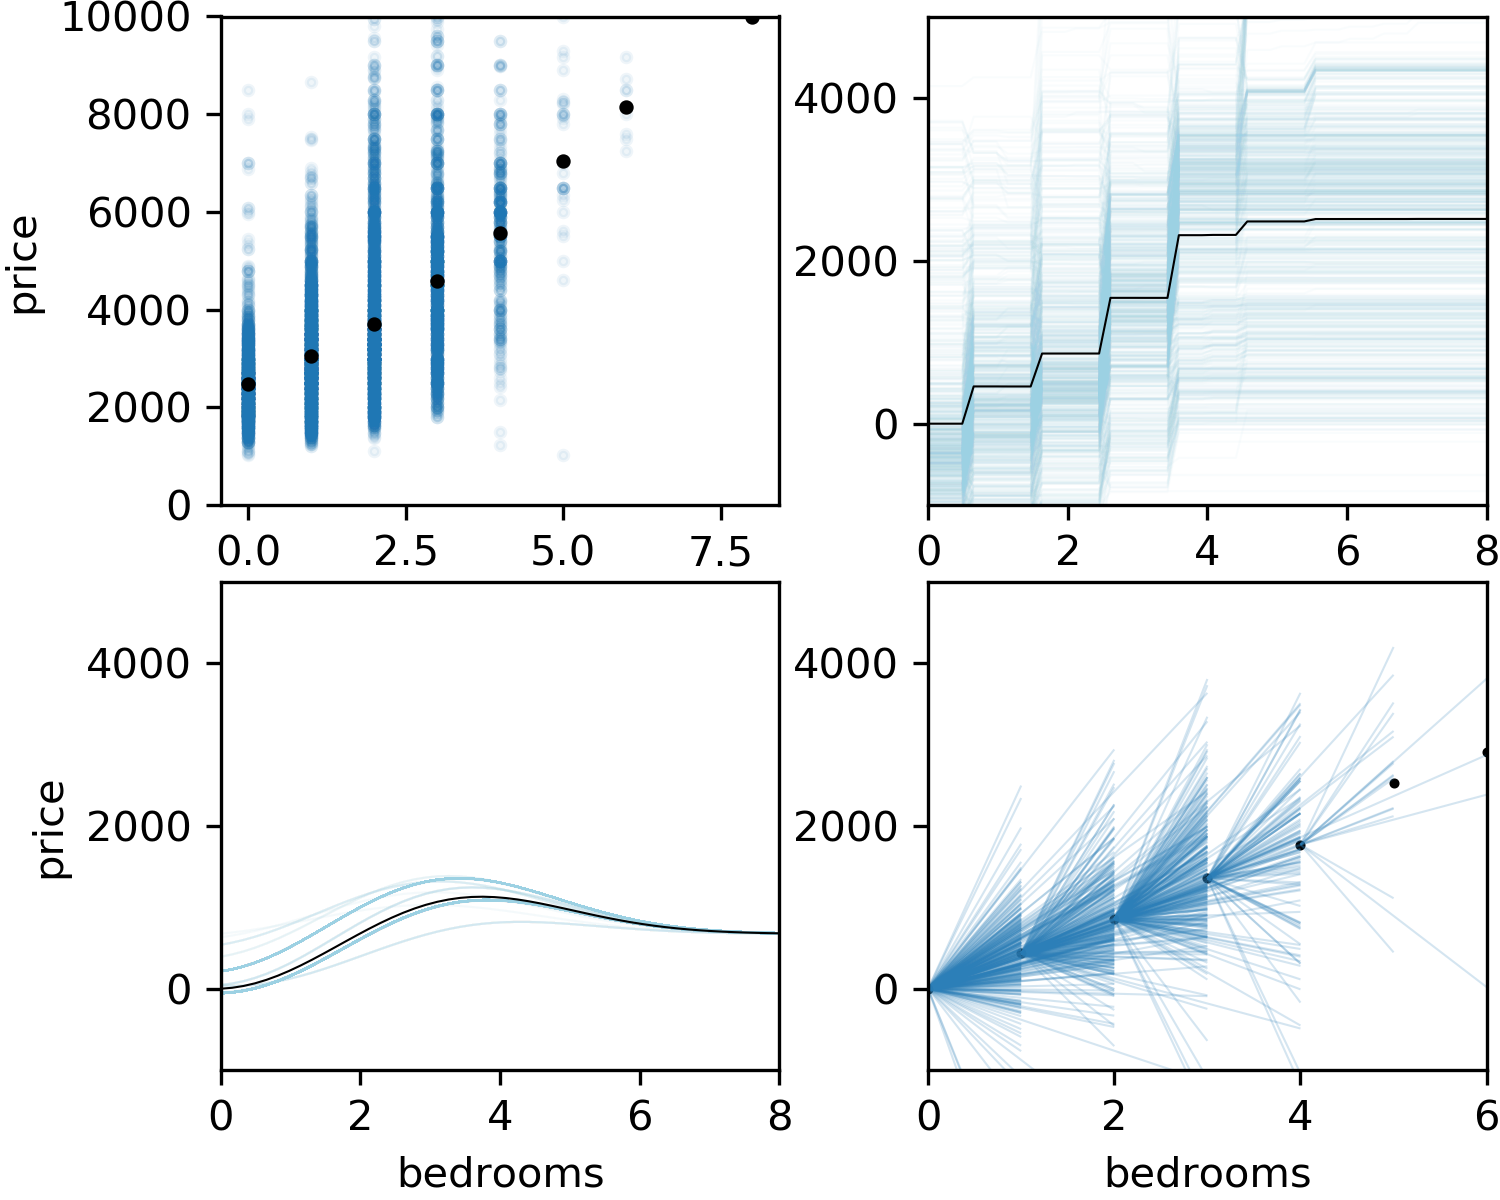
\includegraphics[scale=0.7]{images/bedrooms_vs_price.png}
\caption{{\bf  Marginal plot, PDP/ICE plot, and \spd{} plot of bedrooms versus rent price; sample size 9000 of 400k...{\color{red} we should label these plots}}}
\label{fig:baths_price}
\end{center}
\end{figure}

\cut{The partial dependence plot broadly follows the marginal plot except for the prices of two and three bedrooms apartments, where it levels off. This is counterintuitive and exposes an issue with PD and ICE plots.} While PDP and ICE plots are {\em model-agnostic}, they are not {\em model-independent} and are subject to the strengths and weaknesses of the model making predictions. For example as seen in the left panel of Figure \figref{fig:baths_price}, random forests (RF) do not well extrapolate beyond their training set support range and this data set subset of 10,000 observations has very few apartments with more than 5 bedrooms. (Note the lack of blue dots in that range of the marginal plot.) PDP and ICE plots shift the bedrooms feature of all observations from 0 to 6, accepting less trustworthy predictions from the model in extreme ranges.   

Obtaining radically different PDP and ICE plots for different underlying models is undesirable because users cannot distinguish between interesting target fluctuations and artifacts of their model choice. Consider \figref{fig:baths_price}(c) that shows the PDP/ICE plot for the exact same data set but using a Support Vector Machine (SVM with $\gamma=1/p$). The SVM appears to have difficulty capturing the relationship between bedrooms and price evident from the marginal plot, which means PDP and ICE plots derived from an SVM for this variable are not accurate; plots derived from high-bias models should not be trusted. At the very least, users of PDP and ICE should compare plots derived from multiple models. 

\figref{fig:baths_price}(d) shows the partial dependence of rent on the number of bedrooms (as black dots) using the \spd{} approach described in this paper. The plot also depicts the density of data in the bedrooms/rent space by the number and location of lines, identifies the unique $x$ (bedrooms) values, and characterizes the variability of the slopes across $x$ by the spread of the line angles. {\color{red} Terence - I think we should embellish this paragraph a little more to sell how \spd{} is awesome in comparison to the other strategies.}

There are two remaining issues with PD plots associated with the relationship between features. First, as Friedman pointed out, PD plots are most accurate ``{\em when {\em [the model]} is dominated by low order interactions.}''  Feature interactions, such as $x_1x_2$ in a linear model, are difficult to tease apart to obtain partial dependence on just $x_1$ or $x_2$. \cut{\todo{James: should we remove this parenthetical? Yep!, described in Section 1} (Feature $x_j^T = (x_{1j}, .., x_{Nj})$ is a column vector of the  $n \times p$ explanatory matrix ${\bf X}$).} ICE plots address this issue by showing separate prediction curves for each observation as the feature of interest is moved through all possible values.  This not only shows the variation hidden by the PD average curve, but it depicts interaction relationships between the feature of interest and other features.

The second issue stems from a lack of independence between features.  In a nutshell, not every combination of codependent features is sensible or even possible. For example, in the apartment rent application in Figure 1, there are no apartments with five bedrooms with just one or even zero bathrooms. Similarly, there are no four bathroom studios. Because PDP and ICE alter observations by shifting the feature of interest through all possible feature values, they run the risk of conjuring up nonsensical observations which influence the calculation of partial dependence. In our experience, features in real data sets are very often codependent to some degree. This problem can be mitigated by computing PD and ICE plots on groups of mutually-dependent or interacting features of interest. {\color{red} Ter - not quite sure I understand this mitigation strategy. Can you explain?} \todo{but could involve identifying subsets and computing lots of combinations and we still might want to know about a single contribution.}

\begin{figure}[htbp]
\begin{center}
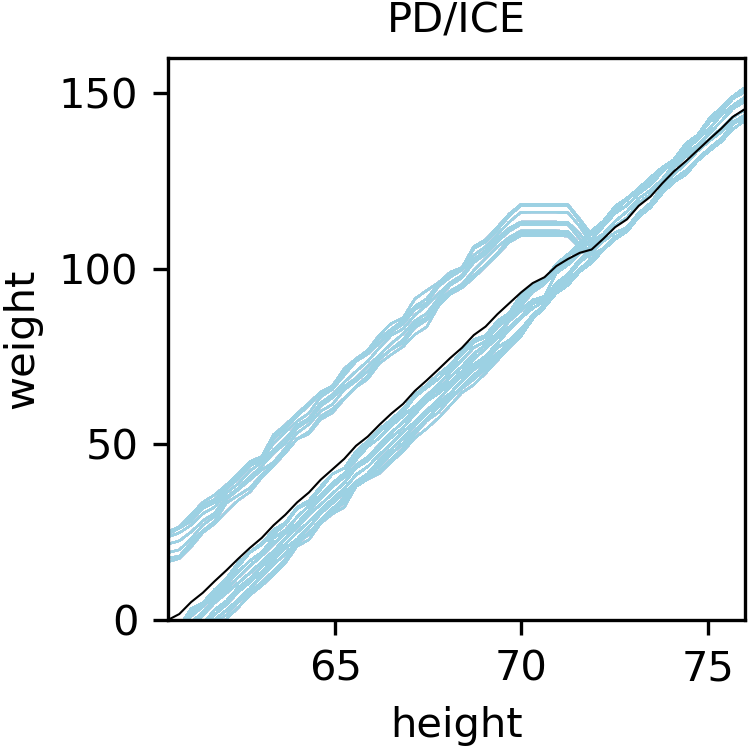
\includegraphics[scale=0.7]{images/height_vs_weight_pdp.png}
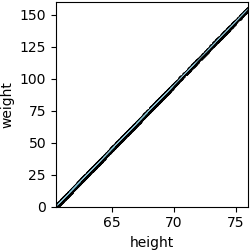
\includegraphics[scale=0.7]{images/height_vs_weight_stratpd.png}
\caption{{\bf  height and educ vs weight}}
\label{fig:height_vs_weight}
\end{center}
\end{figure}

To illustrate how variable codependencies result in misleading PD and ICE plots, consider a body weight data set with observations matching a person's characteristics to a weight in pounds. We discuss the data set details in \secref{sec:codep} (Equation \eqref{eq:weight}), but for the moment, assume that women are slightly shorter on average and are 30 pounds heavier if pregnant. The PD/ICE plot in \figref{fig:height_vs_weight}(a) shows an inaccurate partial dependence where shorter people are slightly heavier per inch of height than those over about 72 inches. At first glance, one may surmise that there is some interesting trend between weight and individuals shorter than 72 inches. The blue ICE lines jump up significantly for shorter heights due to the codependence of $x_{sex}$ and $x_{pregnant}$ because PD and ICE conjure up pregnant males and ask the model to estimate their weight. To be clear, the weight equation has no interaction term with $x_{height}$ and $x_{pregnant}$, but $x_{height}$ is indirectly related to $x_{pregnant}$ (via $x_{sex}$). {\color{red} how can we be sure that this is the case and that the jumps aren't simply because pregnant women, who are typically shorter, have a jump in weight?} The \spd{} plot in \figref{fig:height_vs_weight}(b), on the other hand, is not confused by codependence and gives the true partial dependence of weight on height. 

\todo{needs a transition sentence here}

\section{A stratification approach}

In a perfect world, supporting codependent and interacting features would be straightforward because we would know the actual function, $y = f(X)$ that precisely maps a feature vector $X$ to target value $y$ and in such cases we could directly quantify the relationship between any feature and $y$. Let $c \in \{1, \ldots, p\}$. In general, our proposed \spd{} approach quantifies the relationship between any subset of variables and the response; however for the sake of clarity we will describe the approach in terms of a single feature $x_c$.

\cut{The partial derivative of $f(X)$ with respect to a single variable of interest $x_c$ describes how a unit change in $x_c$ affects $y$ for all $x_c$ values, treating all other variables as constants. Integrating the partial derivative $\frac{\partial}{\partial x_{c}} f(X)$ would yield a curve showing just $x_c$'s contribution to $y$. }

Although $y = f(X)$ is unavailable, a linear regression model of $y$ on the columns of $\mathbf{X}$ provides the general trend of $y$ versus feature $x_c$ via regression coefficient $\beta_c$. For a unit change in $x_c$, $y$ increases or decreases by $\widehat{\beta}_c$, effectively canceling out or controlling for the other features, \xnc. The primary problem with fitting a global linear model lies in the fact it does not capture higher order relationships between $(X,y)$ observation pairs. This is because the coefficient $\widehat{\beta}_c$ is a constant which smooths over any local $y$ fluctuations across the entire range of $x_c$. Varying coefficient models like those introduced in \citet{fan2008statistical} can model such heterogeneities across the range of $x_c$; however, the identified relationships remain correlative and not causal. \cut{Second, linear models require dummy variables to represent (and replace) categorical $x_c$ variables, therefore, regression coefficients would describe the relationship between the presence or absence of a single category and $y$, rather than $x_c$ and $y$. \color{red} Although I agree that categorical variables are an important consideration, many stats folks would not agree with this statement and are perfectly happy with its interpretation.}

A simple approach to assessing partial dependence between $y$ and $X_c$ involves the stratification of the observations into collections in which \xnc{} are the same within each collection. Let $G$ be a group of observations, identified by a set of row indices, where each observation has identical \xnc{} features. For a given $G$, the $\{(x_{ic},  y_i)\}_{i \in G}$ pairs then partially describe how $x_c$ affects $y$, all else being equal. Regressing $y$ on $x_c$ for the observations in collection $G$ yields an approximation of the relationship between $y$ and $x_c$. For each collection $G$, the coefficient $\beta_G$ quantifies this relationship across the domain of $x_c$ in group $G$: $R_G = [\text{min}(x_{ic}), \text{max}(x_{ic})]_{i \in G}$. Because regions from multiple groups could overlap, the partial dependence between $x_c$ and $y$ in a region $R$ is calculated as the weighted average of all coefficients covering that region: 

\begin{equation}\label{eq:truebeta}
	\beta_R = \dfrac{1}{\displaystyle\sum_{G \in R} |G|}\displaystyle\sum_{G \in R}|G|\beta_G,
\end{equation}

\noindent where $|G|$ is the cardinality of the collection $G$. The collection of regions and coefficients, $\{(R, \beta_R)\}_{R \in x_c}$, cover the full $x_c$ range and represent a localized approximation of the partial derivative of the unknown $f(X)$ with respect to $x_c$. In the case of exact stratification on \xnc{}, the estimators $\widehat{\beta}_R$ are unbiased for the true causal effect between $y$ and $X_c$ in region $R$. {\color{red} state this in a proposition? This is simply the Horvitz Thompson estimator for the LOESS curve in the same region (I think). Perhaps we state that as a result and point out that it does not work if we are in high dimensions.}  

Unfortunately, this stratification approach works for two or three variables but breaks down for more variables because it is impractical to find groups of observations that are equal across so many variables, i.e., the curse of dimensionality.  Nonetheless, stratification is simple, well understood, and clearly isolates the effect of $x_c$ on $y$ from the other features, even in the presence of codependent and interacting features.  The only obstacle is a general and practical mechanism for stratifying observations with many variables, which leads us to the primary contribution of this paper.

\subsection{StratPD for numerical variables}

\spd{} seeks to isolate the effects of $x_c$ on the observations $\mathbf{y}$ in the presence of confounding variables. Briefly, \spd{} proceeds in two steps. First, the observations are stratified into disjoint collections of observations $S_1, \ldots, S_m \subseteq \{1, \ldots, n\}$ to ensure that the variables \xnc{} are approximately constant in each $S_j$. The relationship between $y$ and $x_c$ is then approximated using a local linear approximation in each stratum. The partial dependence function $y$ and $x_c$ between on a region $R$ is calculated as the weighted average of the linear relationship between $y$ and $x_c$ over the strata contained in $R$. This is explained in detail next. 
{\color{red} HERE!}
For the stratification step of \spd{}, the key idea is to relax stratification so that it organizes observations into groups of similar rather than equal observations. Our approach, called \spd, trains a decision tree regressor {\color{red} check - decision tree or random forest?}, $T$, as in \cite{CART}, on $(x_{\overline{c}}, {\bf y})$ to stratify observations according to the relationship between \xnc{} and $y$. Each leaf in the tree, $L \in T$, represents a region of \xnc{} space and $(L_x, L_y)$ are the $x_c$ and $y$ observations associated with $L$. \spd{} then characterizes the relationship between $L_y$ and $L_x$ for each $L$ by (i) training another decision tree, $T'$, on $(L_x, L_y)$ to partition $x_c$ space into $(L'_x, L'_y)$ for each $L' \in T'$ and (ii) fitting a simple linear regressor to each subregion $(L'_x, L'_y)$.  The collection of $\beta_{L'}$ coefficients represent the localized slope across the $x_c$ space of $L$. Ignoring the $y$-intercepts removes the contribution of \xnc{} to $y$ in $L'$.

The regions of $x_c$ spanned by the various $\beta_{L'}$ generally overlap and the slope in any region, $R$, is the weighted average of all $\beta_{L'}$ that overlap $R$:

\begin{equation}\label{eq:slope}
\beta_R = \frac{1}{\displaystyle\sum_{L' \in R} |L'|}\displaystyle\sum_{L' \in R}|L'|\beta_{L'}
\end{equation}

Slope $\beta_R$ is an estimate of the partial derivative across the region $R$, and so numerically integrating the partial derivatives across $x_c$ space gives a curve representing the contribution of $x_c$ to $y$.  Algorithm 1 encodes the \spd{} process and the full Python 3 source code is available at {\small \url{https://github.com/parrt/stratx}}. \figref{fig:leaves} depicts the averaging and integration process.  

\begin{figure}[htbp]
\begin{center}
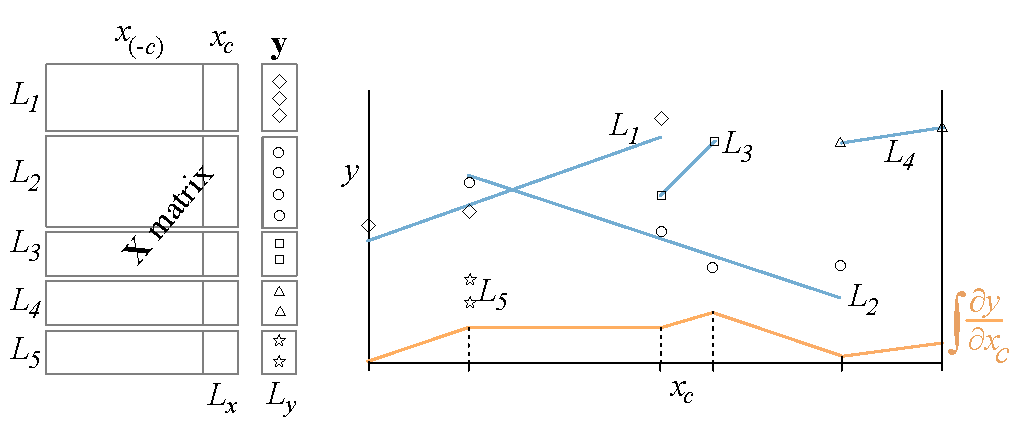
\includegraphics[scale=0.7]{images/leaves.pdf}
\caption{BLORT There are five leaves, $L_1 .. L_5$, with regression lines fit through leaf observations. The $x_c$ values in $L_5$ are identical so its infinite slope is ignored.}
\label{fig:leaves}
\end{center}
\end{figure}

\cut{
\spd{} trains a decision tree in the usual way but on $(x_{\overline{c}}, {\bf y})$ rather than $({\bf X}, {\bf y})$. Observations $(X_i, y_i)$ that end up in a tree leaf are, by definition, in the same region of \xnc{} feature space. Training greedily partitions feature space in order to minimize variance of $y_i$ within regions, which partitions feature space into tighter and tighter regions.  (The collection of variable inequality decision nodes along the path from from root to a leaf demarcates the region of feature space.) Tighter regions imply more similar \xnc{} values, which means $x_c$ is likely responsible for any variation in $y$; this likelihood decreases as the size of $L$ increases.  The training process must leave at least two samples per leaf in order to fit a localized linear model.  
}

Revisiting the \spd{} plot in \figref{fig:height_vs_weight}(d), derived from the apartment rent data set, each blue line represents a local slope $\beta_L'$ through the observations in $L'$ (which is a partition of $x_c$ space whose \xnc{} features are similar). Lines extend from the minimum to maximum $x_c$ value in $L'$.  Because we are interested in the relative contribution of $x_c$ to $y$, \spd{} plots use zero as a $y$-axis baseline. The black dots represent the integration of the partial derivative estimates up to and including each unique $x_c$ value (except the first $x_c$, whose integral value is 0). The partial derivative estimate at an $x_c$ value is the (weighted) average slope of the blue lines emanating from that value. \spd{} does not interpolate between $x_c$ points and so the plot shows dots not lines. 

Partial dependence through stratification also works for data sets with categorical variables in \xnc{}, given a suitable similarity measure between observations that supports categorical variables, but identifying an appropriate categorical similarity measure is a well-known issue.  Decision trees, however, support categorical variables easily and effectively by treating categories as unique integers. Observations with categorical variables that end up in the same leaf lie are likely to be similar (\cite{RFunsup}). Algorithm 1, therefore, works without modification for \xnc{} containing categorical variables. When the column of interest, $x_c$, is categorical, however, a new algorithm is required.

\subsection{CatStratPD for categorical variables}

The stratification approach can also capture how a categorical variable $x_c$ affects $y$, instead of just a single category at a time (if one were forced to dummy-encode $x_c$). As with \spd{}, the \cspd{} algorithm stratifies $\bf X$ into groups of similar \xnc{} features by training a decision tree regressor on $({\bf X}, {\bf y})$, yielding a collection of leaves. But, because categorical variables can be unordered nominal variables, the notion of $y$ slope is not meaningful between two categories. Instead of partitioning the $x_c$ space in each leaf $L$, \cspd{} groups leaf observations $(L_x, L_y)$ by the categories in $L_x$ and computes the average $L_y$ value per category.  To erase the $y$-contributions of \xnc{}, \cspd{} subtracts the minimum of the $L_y$ means from all category averages, leaving a relative increase or decrease in $y$  for each category. Then, to get the overall contribution of $x_c$ to $y$ for category $cat$, \cspd{} averages the leaf contributions for $cat$ from all $L$ weighted by $|L|$. See Algorithm 2.

\figref{fig:state_vs_temp}(b) illustrates \cspd{} operating on a categorical variable, $x_{\it state}$, in a synthetic weather data set with data from four states over three years. Temperature data varies in sinusoidal fashion over the year with $N(-5,5)$ noise and different baseline temperatures per state, as the marginal plot in \figref{fig:state_vs_temp}(a) shows. To get the partial dependence of temperature on $x_{\it state}$, \spd{} stratifies by $x_{\it dayofyear}$ and $x_{\it year}$ then groups these similar time buckets by $x_{\it state}$ and computes the average temperature; each blue dot represents a leaf average. The overall temperature estimate per state is the average of those leaf averages, represented by a solid black dash. We use a strip plot to exhibit the variation and density of $y$ values per category. The \cspd{} plot accurately identifies the baseline temperature per state, as does the PD/ICE plot in \figref{fig:state_vs_temp}(c).

\begin{figure}[htbp]
\begin{center}
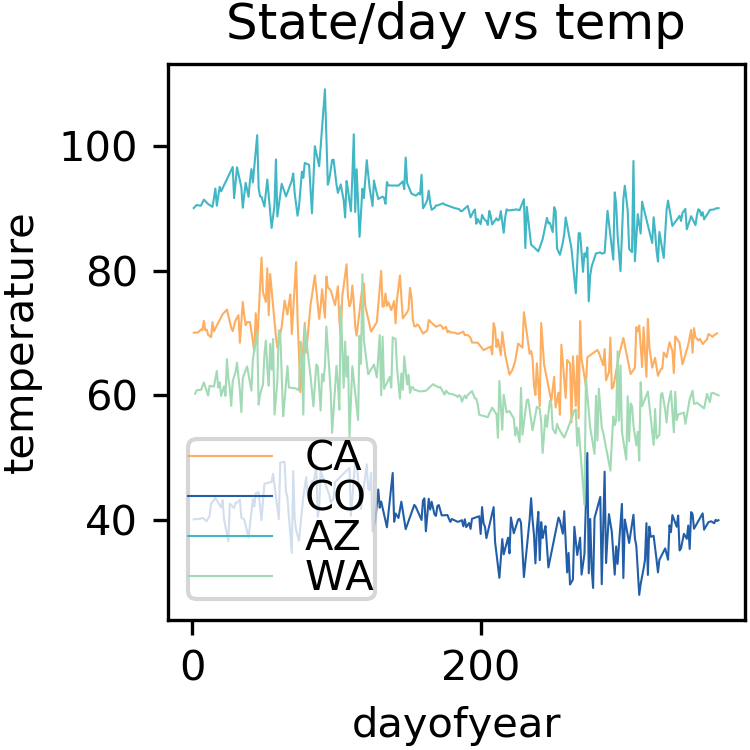
\includegraphics[scale=0.7]{images/dayofyear_vs_temp.png}
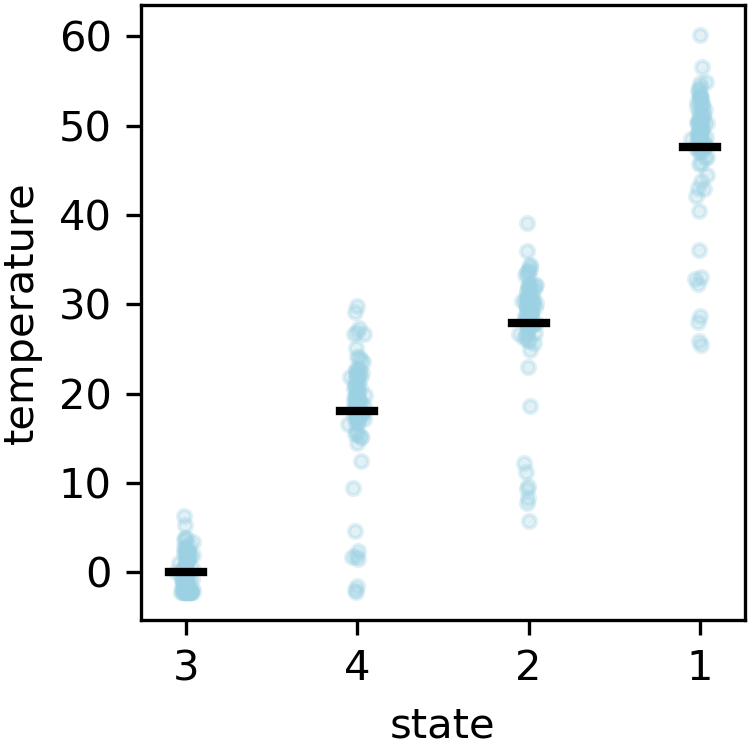
\includegraphics[scale=0.7]{images/state_vs_temp_stratpd.png}
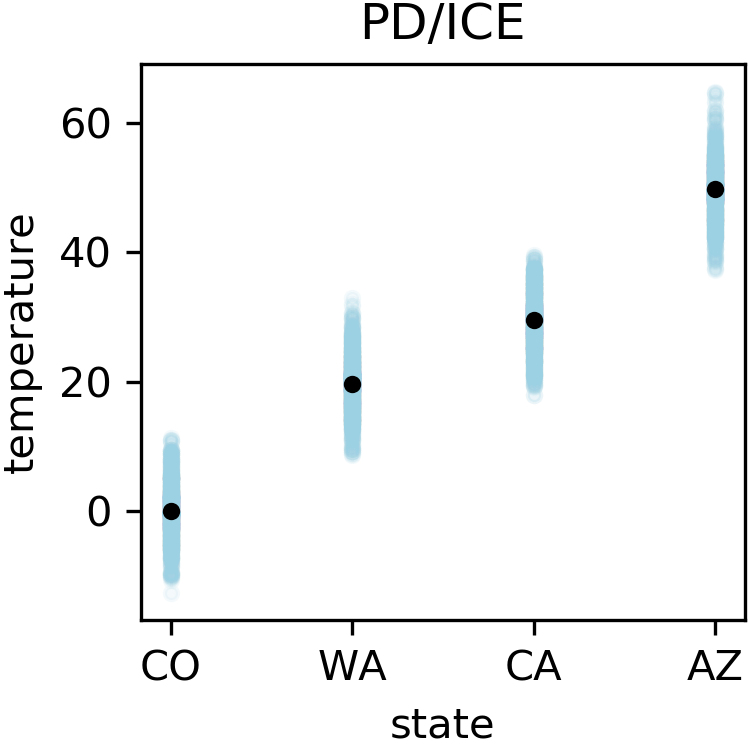
\includegraphics[scale=0.7]{images/state_vs_temp_pdp.png}
\caption{{\bf  state  vs temp}}
\label{fig:state_vs_temp}
\end{center}
\end{figure}

\subsection{Partitioning feature space with trees and forests}

Stratification of $(x_{\overline{c}}, y)$ into regions of similar observations is at the core of our approach so it's worth examining how \spd{} partitions feature space in more detail.  The goal is to find groups of extremely similar \xnc{} values in $({\bf X}, {\bf y})$ so fluctuations in $y$ are due solely to changes in $x_c$. Such groups yield pieces of the partial dependence of $y$ on $x_c$. \spd{} looks for similar observations because, beyond a few variables, it's not possible to stratify observations by equal \xnc{} values. 

Inventing a new partitioning strategy is unnecessary because decision trees already exist that can tesselate \xnc{} feature space into small hypervolumes of similar observations. If a hypervolume is tight enough, then \xnc{} values are very similar and the slope of a regression line through $(L_x, L_y)$ is a good estimate of the partial derivative of $\frac{\partial y}{\partial x_{c}}$ in that region.  If the volume for leaf $L$ is too large, then \xnc{} observations in $L$ are not similar enough to conclude that changes in $y$ are due to $x_c$ alone. By default, our Python implementation of \spd{} creates decision trees with at least 10 observations per leaf, but depending on $y$, post-training leaf size is unbounded. The $x_c$ space within each leaf is then partitioned using another decision tree in preparation for piecewise linear approximation.

Decision trees are known to overfit, which was the impetus for the invention of Random Forests(tm) (RF) \cite{RF}.  The use of decision trees rather than RFs in \spd, therefore, seems an odd choice. Using RFs was our initial approach and the \spd{} algorithm and source code still supports them. (The only change required to support RFs is to iterate over all leaves from all trees, rather than the leaves of a single tree, to collect $\beta_L$ slopes.)  Decision trees are sufficient for partial dependence, however, because the goal is to understand the population described by the training set, not to make predictions; that is what models are for. The one exception is that multiple trees are needed to handle features in \xnc{} that are identical or highly-correlated with $x_c$ (see \secref{sec:dup}).

To reduce overfitting, RFs bootstrap and select split variables from a subset of all variables in order to create uncorrelated trees. But, that means increasing bias to some degree because each tree is trained on roughly 2/3 of the training data and without considering some of the variables. Because our goal is to group together {\em all} observations that are similar in {\em all} \xnc{} variables, it is counterproductive to bootstrap and select variables from a subset. Because partial dependence is meant to explore existing $(\bf X, y)$ data rather than future data, there's no point in sacrificing accuracy for the sake of generality. 

For the data sets we examined during the preparation of this paper, moving from a decision tree to a random forest of various sizes did not affect the partial dependence results; \figref{fig:weight_ntrees} and \figref{fig:rent_ntrees} show some typical results. The integrated partial derivative curves identified by the black dots do not change as the number of trees increases from left to right.  In one simulation run for the rent data set, we did see a difference in the partial dependence dots for an extreme value of $x_{bedrooms}$ with very few $y$ values, but it's unclear which plot is correct for this real data set. (The answer is unclear because the true partial dependence for a variable of an unknown function is unknown.)

The blue lines representing piecewise partial derivative estimates increase in number as the number of partitions (leaves) increases.  Note that the variance of the partial derivative estimates is wider for RFs than for a single decision tree. This is expected because the decision tree leaves contain all observations in a feature space hypervolume and so the estimate will be less biased; RF leaves have at most 2/3 of the observations for the same hypervolume, the bootstrapping population size estimate. The education versus weight plots in \figref{fig:weight_ntrees} illustrate this most clearly. The blue ``cone'' around the partial dependence dots widens as the number of trees increases.  

Increasing the number of trees does not improve accuracy and increases the time complexity linearly in the number of trees, which is roughly what we see in practice.  For example, using a single decision tree to partition a 9,000-observation rent data set sample and generate a plot takes 1.5s on our 4.0Ghz processor but about 50s for 30 trees (first row, far right of \figref{fig:rent_ntrees}). \todo{seems less accuarate with bootstrap}

\begin{figure}[htbp]
\begin{center}
% 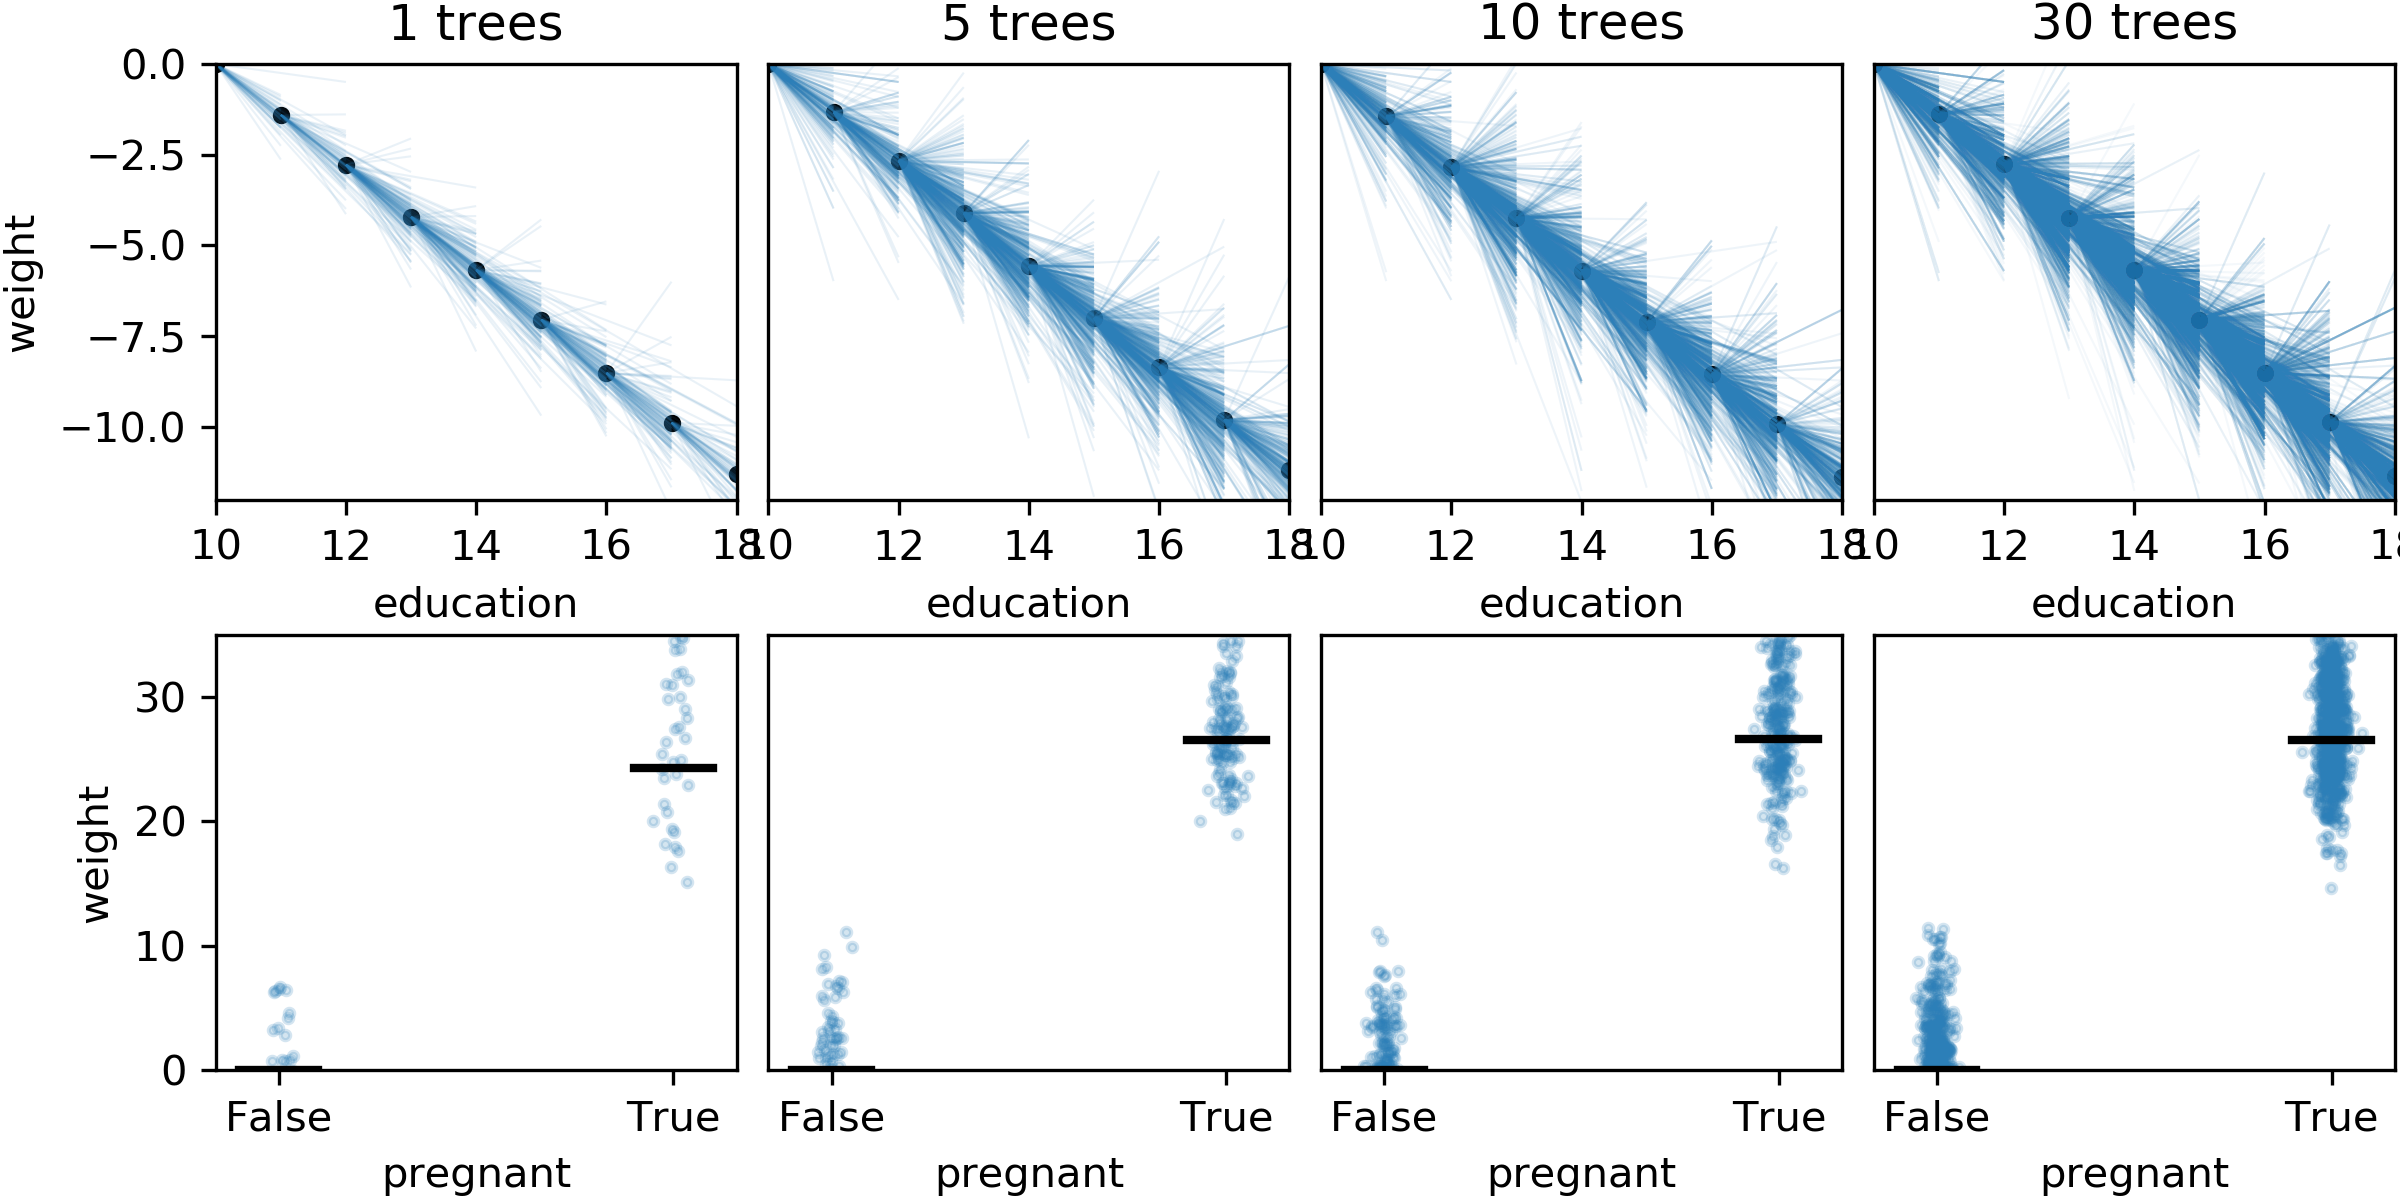
\includegraphics[scale=0.5]{images/education_pregnant_vs_weight_ntrees.png}
\caption{{\bf  weight ntrees 1, 5, 10, 30 trees; ${\it min\_samples\_leaf\_partition}=5$}}
\label{fig:weight_ntrees}
\end{center}
\end{figure}

\begin{figure}[htbp]
\begin{center}
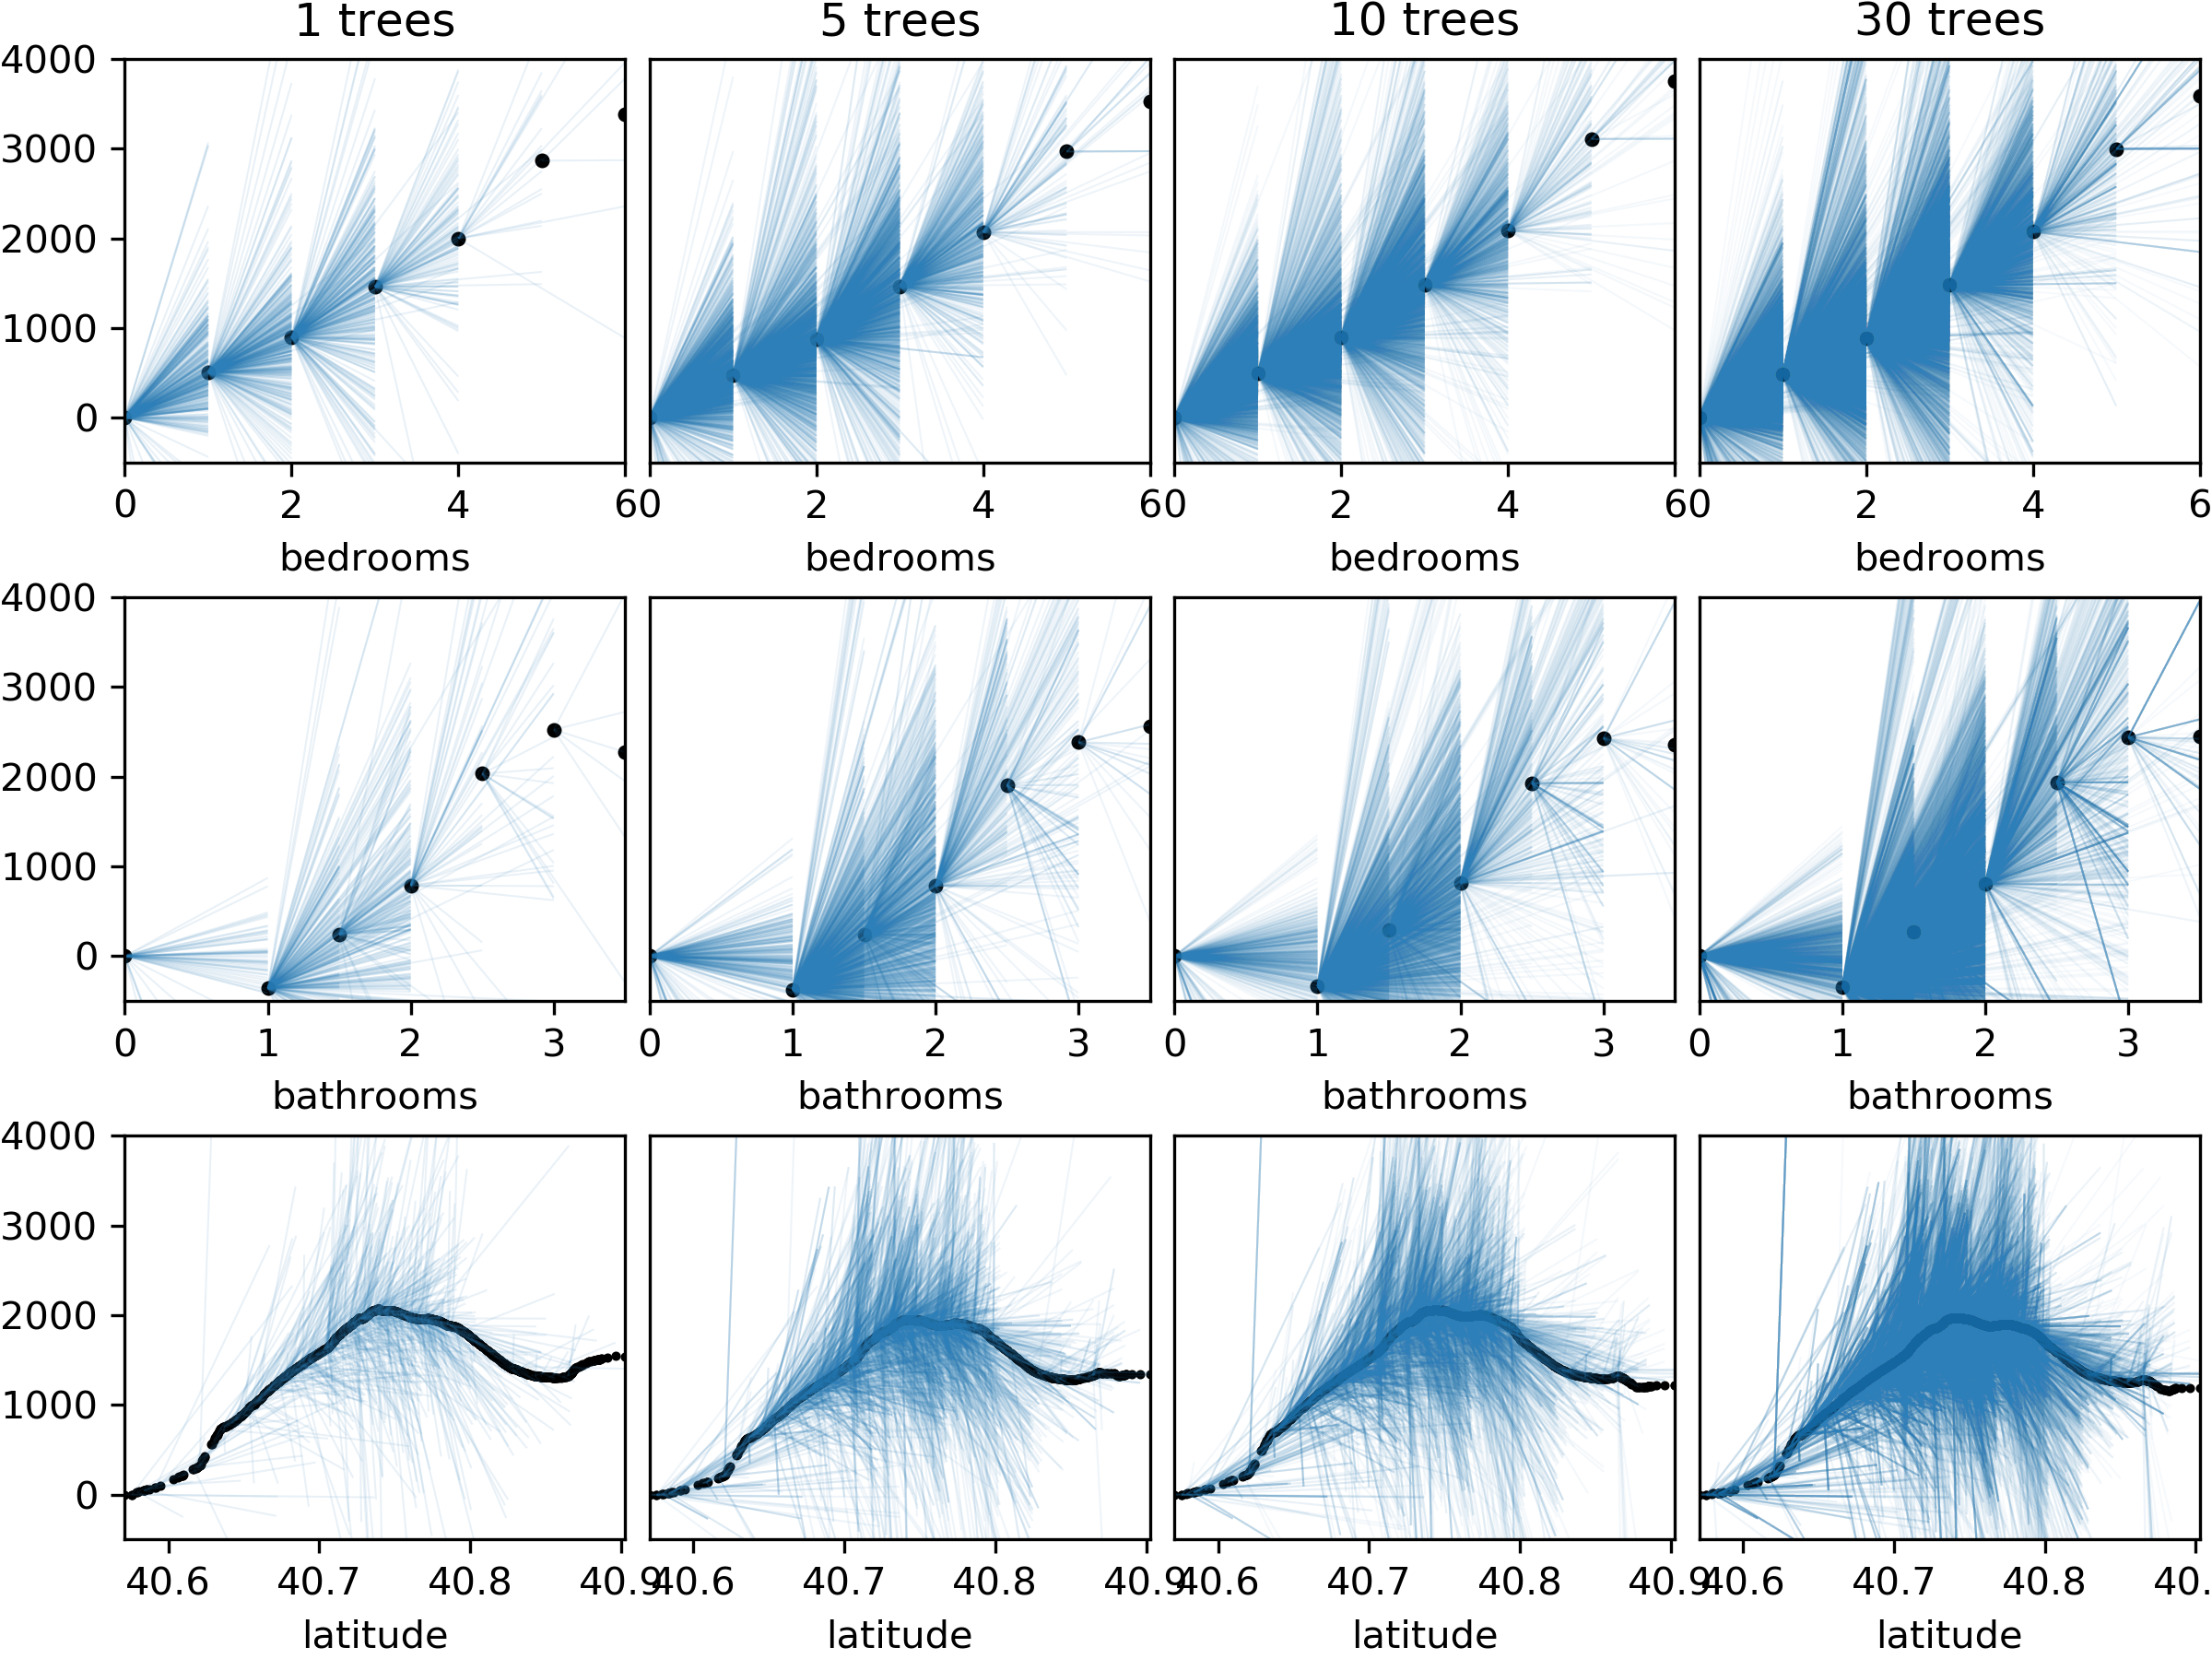
\includegraphics[scale=0.5]{images/rent_ntrees.png}
\caption{{\bf  rent ntrees 1, 5, 10, 30 trees}}
\label{fig:rent_ntrees}
\end{center}
\end{figure}

Decision trees choose feature space hypervolumes that minimize the variance in $y$, but $y$ is technically not needed to partition \xnc{} into similar regions. \cite{RFunsup} described how to use random forests in an unsupervised fashion by considering the original $\bf X$ matrix as class 1 and a synthesized $\bf X'$ as class 2, which works equally well for individual decision trees, at least for this stratification application. $\bf X'$ is just $\bf X$ with each $x_j$ column permuted, effectively sampling from the $x_j$'s marginal distributions. \figref{fig:rent_weight_unsup} shows typical results from three variables from the rent data set and two variables from the synthesized weight data set.  The left column shows unsupervised partitioning of $\bf X$ and the right column shows the usual supervised partitioning with $(\bf X, y)$. The results are very similar but the variance of the partial derivative estimates for the unsupervised case appears to be a bit wider. The \cspd{} unsupervised and supervised plots for categorical variable $x_{\it pregnant}$ in \figref{fig:rent_weight_unsup}(b) are virtually indistinguishable to the eye. 

\figref{fig:boston_unsup} illustrates a case where unsupervised partitioning is less stable: $x_{\it AGE}$ versus $x_{\it MEDV}$ (median house value) from the well-known Boston housing data set. The figure shows a marginal plot then the unsupervised and supervised \spd{} plots (and finally the PD/ICE plot). To stabilize the unsupervised version, we used 20 trees with bootstrapping. But, in the end, there's no reason to perform unsupervised partitioning when $y$ is always available. (Partial dependence makes no sense without $y$.) 

The point is that partitioning \xnc{}  with a decision tree is more about $\bf X$ than $\bf y$, which strengthens our claim of model-independence. \spd{} does not rely on a user's model, never makes predictions from internal models, and can even get away with partitioning feature space without $\bf y$.

\begin{figure}[htbp]
\begin{center}
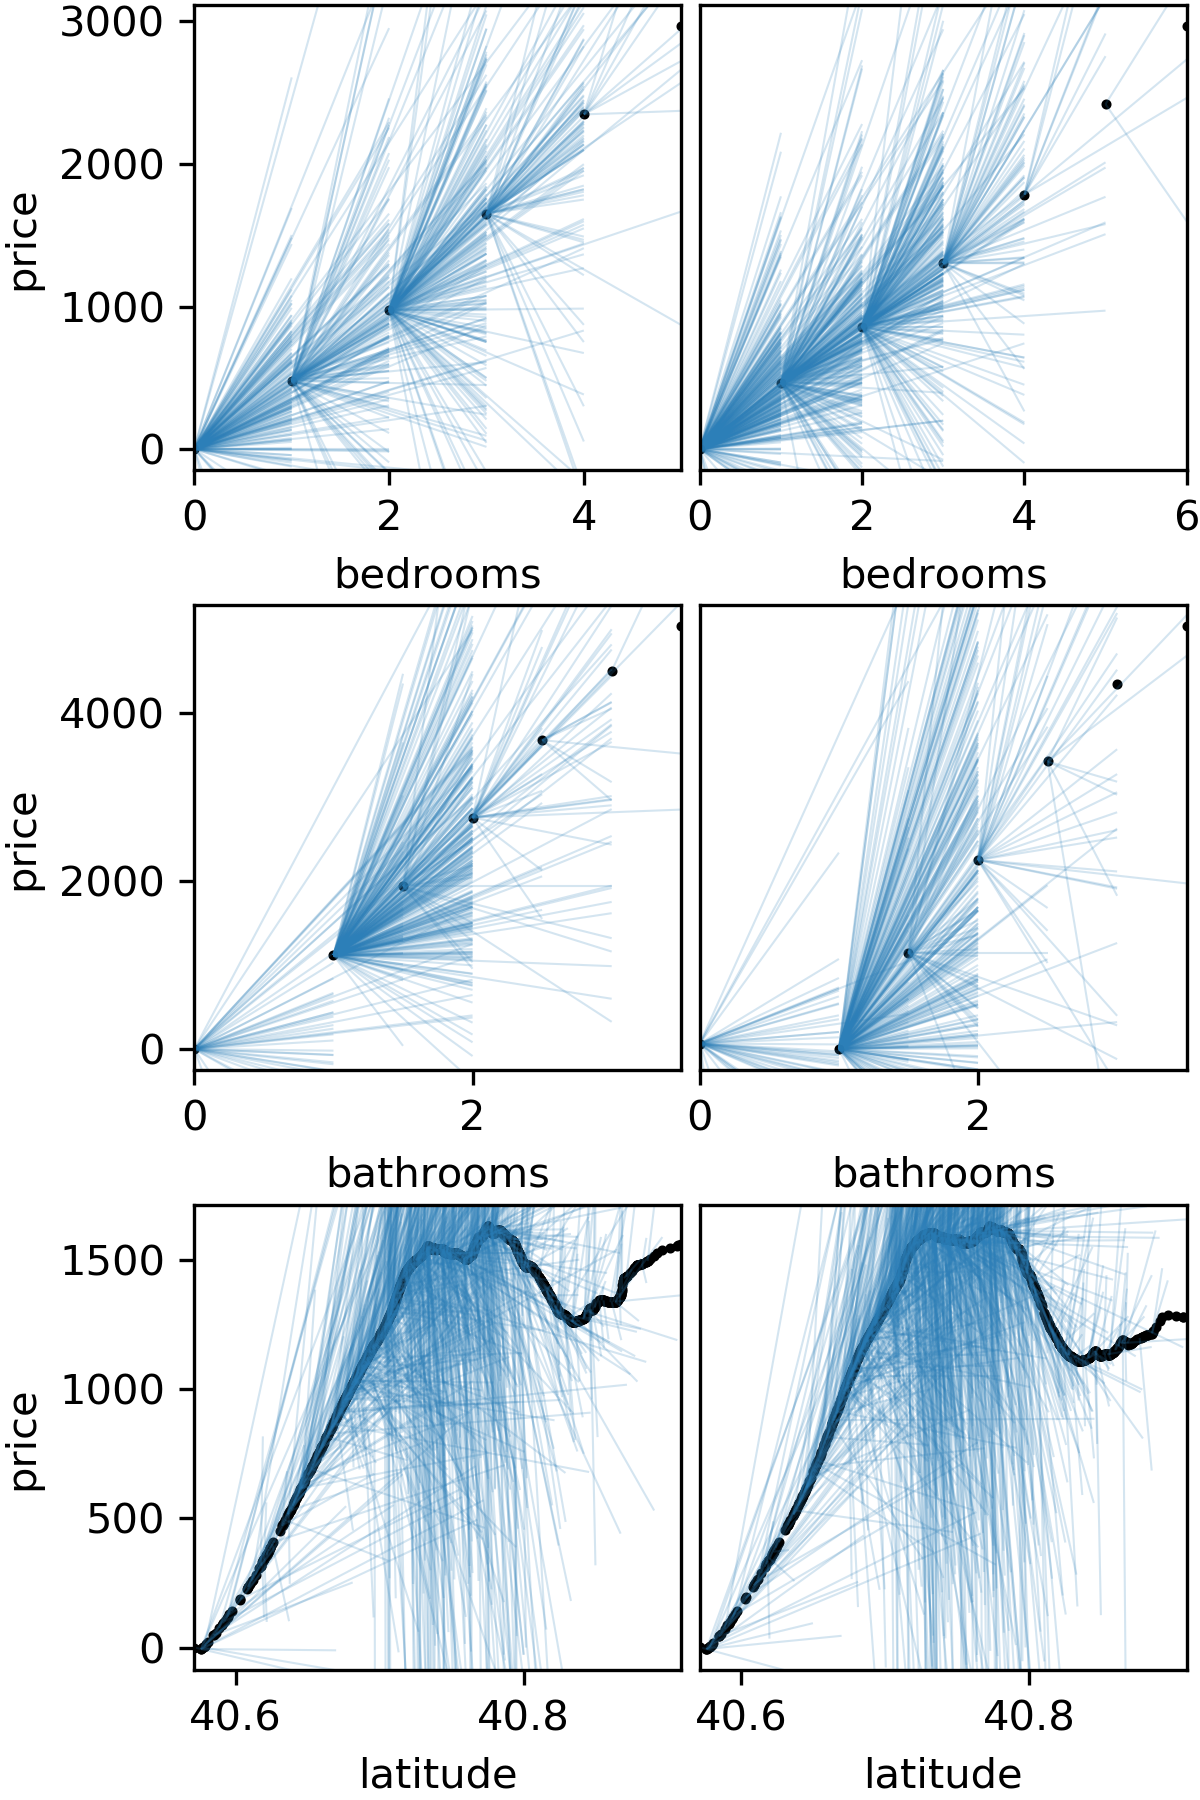
\includegraphics[scale=0.7]{images/rent_unsup.png}
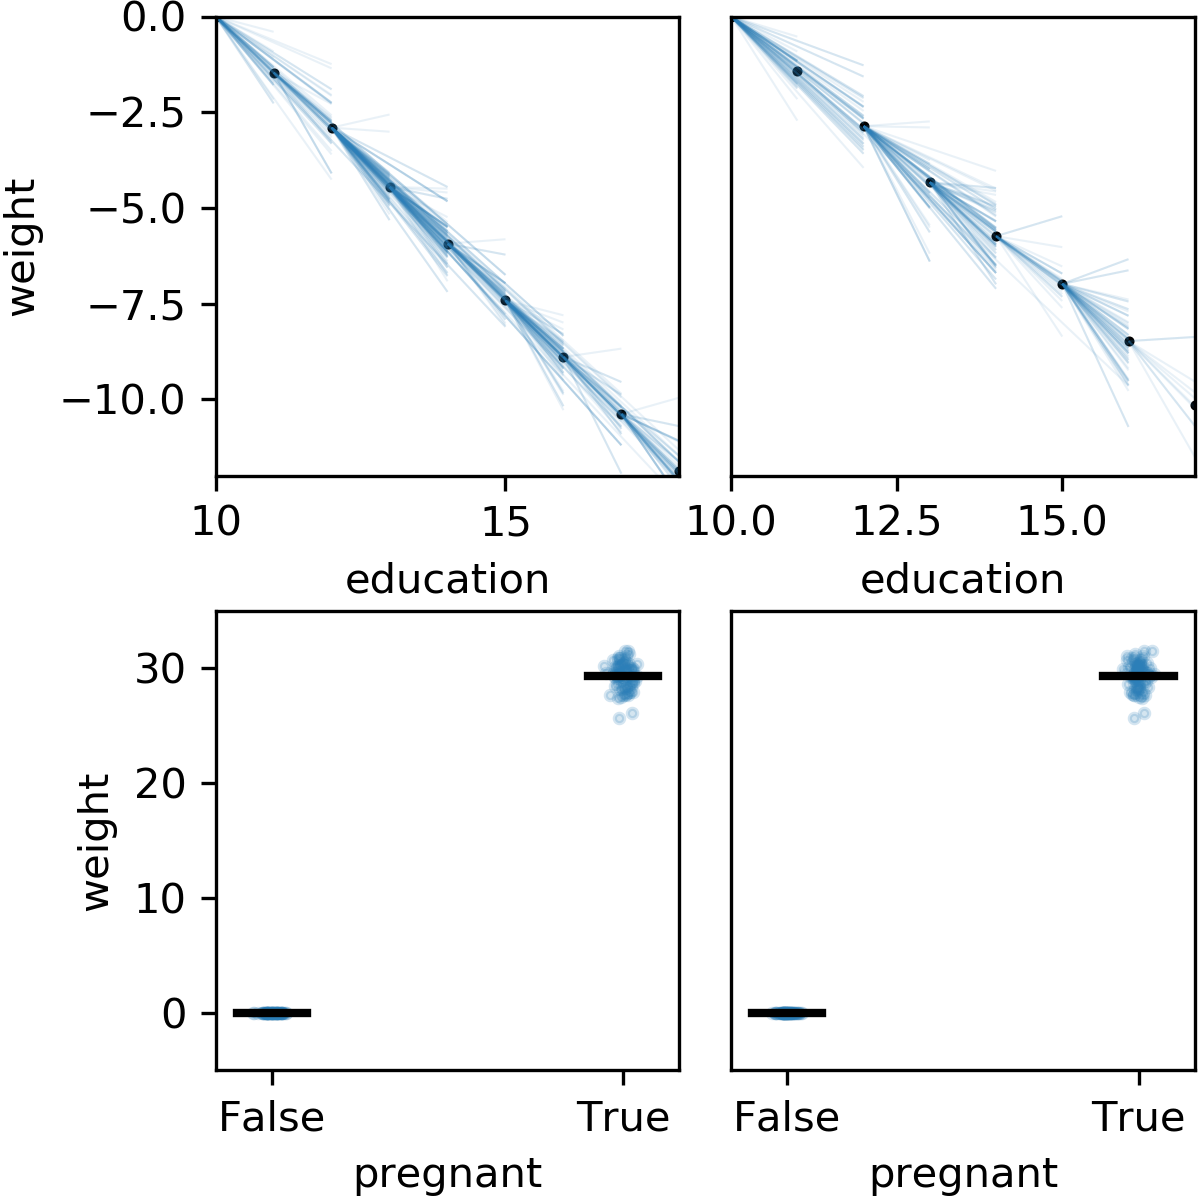
\includegraphics[scale=0.7]{images/weight_unsup.png}
\caption{{\bf  rent and weight unsupervised}}
\label{fig:rent_weight_unsup}
\end{center}
\end{figure}

\begin{figure}[htbp]
\begin{center}
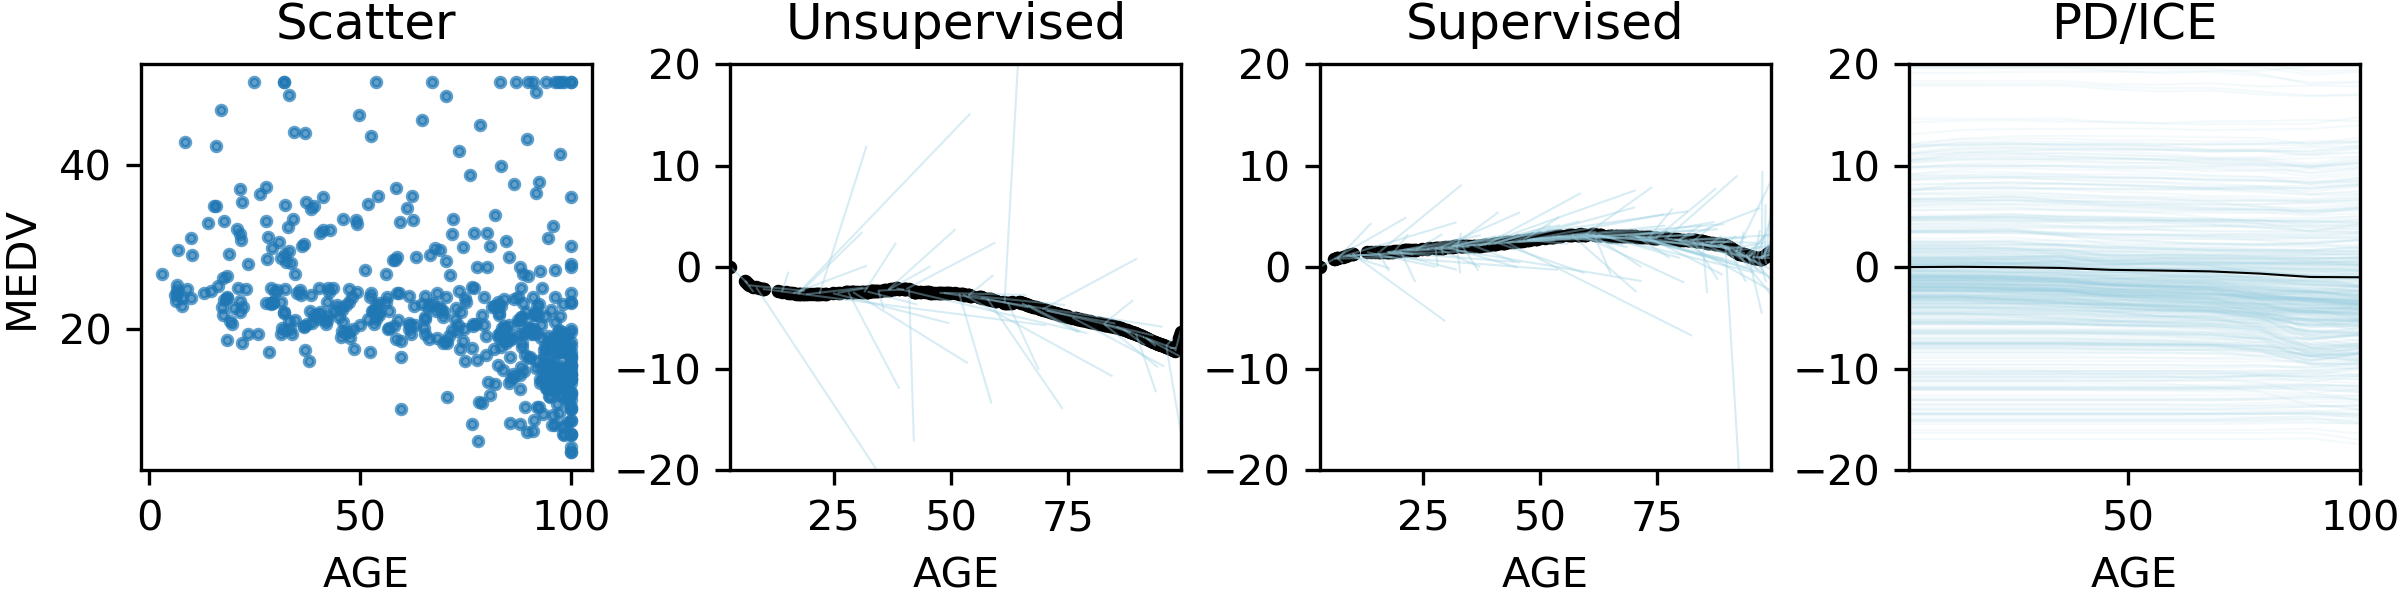
\includegraphics[scale=0.7]{images/boston_unsup.png}
\caption{{\bf   Boston unsup}}
\label{fig:boston_unsup}
\end{center}
\end{figure}

\todo{where does this go? \spd{} degenerates to a simple marginal plot if training yields a tree with a single leaf node containing all of \xnc{}. what are degenerate cases? approximation error.}

\section{Related Work}\label{sec:related}

The PDP and ICE methods mentioned in this paper each rely on the practitioner first estimating $f$ with some machine learning model before estimating partial effects. Given a fitted model $\widehat{f}$, PDP and ICE estimate the partial effect between $x_C$ and the fitted model $\widehat{f}$. 

PDP seeks to estimate the partial dependence function $\widehat{f}^{PDP}_C(x_C)$ given by

\begin{equation*}\label{eq:PDP} \widehat{f}^{PDP}_C(x_C): = \mathbb{E}_{\overline{C}}\left[\widehat{f}({X})\right] = \int \widehat{f}({X}) d\mathbb{P}(X_{\overline{C}}).\end{equation*}


The function $\widehat{f}_C(x_C)$ describes the average marginal effect that the features $X_C$ has on the prediction $\widehat{f}$. The partial dependence of $X_C$ is a global representation of variable dependence and averages over any heterogeneous relationships between $\mathbf{y}$ and $x_C$. 

The individual conditional expectation (ICE) plot from \cite{ICE} is a local method which estimates the partial dependence of the prediction $\widehat{f}({X})$ on $x_C$ across individual observations. Suppose that $(X_{C_i}, X_{\overline{C}_i})$ are the values of the $i$th row of $\mathbf{X}$. For each $i$, the ICE plot produces a curve from the fitted model over all values of $X_C$ while holding $x_{\overline{C}_i}$ fixed. In particular, for observation $i$ the following curve is plotted $\widehat{f}^{(i)}_C = \widehat{f}((\{X_{C_i}\}_{i = 1}^n, X_{\overline{C}_i}))$. Unlike PDP, ICE can be used to  identify heterogeneous relationships between the fitted model and the features of interest $X_C$. By construction, the PDP curve for a variable $X_C$ is the average over all ICE curves for that variable. In practice, typically both ICE and PDP are used to describe the partial dependence of $\mathbf{y}$ on $X_C$.

An important limitation of PDP and ICE is that they require independence of the features in $\mathbf{X}$. This is rarely the case in practice, and in such situations these plots lead to faulty inference and misinterpretation (see \cite{apley2016visualizing} for a discussion). \cite{apley2016visualizing} introduced the accumulated local effects (ALE) strategy to overcome the independence limitation. The ALE plot is an average partial dependence of $X_C$ on $\widehat{f}$ that is calculated through the accumulation of local changes in the prediction for small windows of $X_C$. Local changes are measured as gradients of $\widehat{f}$ with respect to $X_C$ while $X_{\overline{C}}$ is held fixed. Although the ALE plot is unbiased in the presence of codependent features, it still has some disadvantages. Unlike \spd{}, ALE is not directly suitable for categorical variables as an ordering of each variable is needed for the calculation of gradients of $\widehat{f}$. Furthermore, the user must determine the number of intervals to use for calculating an ALE plot, and there is no general advice on how to do this.

%LIME
\cite{ribeiro2016should} proposed the local interpretable model-agnostic explanations (LIME) method as a strategy to interpret machine learning predictions. For a prediction of interest, LIME learns an interpretable model, on a small neighborhood of data around that prediction that explains the relationship between variables and the response locally. In contrast to \spd{}, LIME is used to create local interpretable models for each prediction; however, it does not directly assess the partial dependence of the response on a subset of variables. Like LIME, \spd{} also relies upon local interpretable models; however, \spd{} does this to explain partial dependence relationships rather than correlative relationships between the response and features. 

%Shapley
The Shapley strategy, introduced in \cite{lundberg2016unexpected}, is a permutation-based method for estimating the relationship between ${y}$ and a variable $X_C$ through a fitted model $\widehat{f}$. In this method, the marginal effect of $X_C$ is represented by the Shapely value, which is the average change in the prediction made from the original data $\widehat{f}$ and the prediction made when all other variables $X_{\overline{C}}$ have been randomly shuffled in the dataset. The permuting of $X_{\overline{C}}$ is repeated many times and the average Shapely value is reported as the importance. Like PDP, ICE, and ALE, the Shapely strategy is also dependent on the machine learning model fitted. Further, like any permutation method, this strategy can suffer from nonsensical observations due to the permuting of $X_{\overline{C}}$, which are subsequently incorporated in the estimated dependence. This is especially problematic in the case of highly correlated features. Finally, a major disadvantage of the Shapely strategy is its computational complexity due to repeated permutations. 

{\color{red} Add partial effects and LOESS?}

{\color{red} Causality?}

% $$\widehat{f}^{ALE}_C(x_C): = \int_{z_o}^{x_C}\mathbb{E}_{\overline{C}|C}\left[\dfrac{\partial \widehat{f}(\mathbf{X})}{\partial x_C} | x_C = z\right] dz = \int_{z_o}^{x_C}\int_{x_{\overline{C}}} \dfrac{\partial \widehat{f}(\mathbf{X})}{\partial x_C} \mathbb{P}(x | z)dxdz, $$
%Put a plot of ICE, PDP, and ALE, econometric stuff, 
% \noindent where $\mathbb{P}(x | z)$ is the conditional distribution of $x_{\overline{C}}$ given $x_C$.


% To summarize the hazards of PD and ICE plots, (i) both are strongly affected by the model chosen by the user, (ii) to obtain accurate plots, PD and ICE rely on the accuracy of the underlying model, which might sacrifice local accuracy to minimize some global loss function. Both plots display model prediction results rather than the data itself. (iii) The potentially inaccurate model feeds off of potentially nonsensical, synthesized observations arising from variable codependencies. What we need is an accurate mechanism that does not rely on, nor make predictions from, a user's model and a mechanism that does not assume mutually independent features.


% PDP math shows that features added or multiplied times the remaining F approximation completely describe the partial dependence; I assume that means that interactions are not a problem.

% Most importantly, \spd{} is model-independent in the sense that it does not expect nor rely on a user's model trained on $({\bf X}, {\bf y})$.  \spd{} does, of course, use models internally: a random forest for stratification and multiple linear models for estimating local partial derivatives.  The biggest difference is that \spd{} does not use predictions from any these models, which means prediction accuracy is irrelevant.  (\todo{refer to unsupervised learning trick}.)  In contrast, PD and ICE rely completely on the model supplied by the user and its accuracy.  Some implementations lay a grid across $x_c$'s range and, therefore, potentially make predictions based upon values not present in $x_c$. Also, as discussed, PD and ICE potentially conjure up nonsensical ${\bf }_i$ feature vectors, due to codependencies, and incorporate resulting predictions into plots.
%
%
%
% do we need to talk about LIME? http://arxiv.org/pdf/1602.04938v1.pdf ?Why Should I Trust You?? Explaining the Predictions of Any Classifier.
%
% there are other ways to stratify X, such as quartiles or binning of some kind but we have to choose the bins or the similarity measure.
%
% talk about how we do not presume independence of features
 
\section{Experimental Results}\label{sec:applications}

This paper proposes a stratification approach to isolating the effect of $x_c$ on target $y$ and has shown a few \spd{} and \cspd{} plots to highlight their advantages over PD and ICE plots. In this section, we provide more examples on synthetic and real data sets, investigate the effect of noisy data, and examine how \spd{} deals with edge cases arising from unusual \xnc{} partitioning.  All plots, including the PD/ICE plots, were generated using the Python {\tt stratx} library and script {\tt genfigs.py} in the github repository generated all figures in this paper. (PD/ICE plots were derived from random forest models with 100 trees and minimum samples per leaf of 1). 

We begin by reproducing graphs from \cite{ICE}, starting with their equation in which independent variables $x_2$ and $x_3$ interact:

\begin{equation}\label{eq:bigX}
y = 0.2x_1 - 5x_2 + 10x_2\mathbf{1}_{x_3 \geq 0} + \epsilon~~~~~x_1, x_2, x_3 \sim U(-1,1), \epsilon \sim N(0,1)
\end{equation}

\noindent \figref{fig:bigx_stratpd} shows the \spd{} plots in the left column for $x_2$ and $x_3$ and the PD/ICE plots in the right column. (1000 observations were drawn.) As \cite{ICE} points out, the PD plot (top row, right side) for $x_2$ shows no effect of $x_2$ on $y$ predictions, but the ICE plot makes it clear that the apparent lack of PD effect is due to an interaction or interactions with other variables that cancel out. In this case, we know from Equation \eqref{eq:bigX} that $x_3$ ``turns off'' $10 x_2$ roughly half the time ($x_3 \sim U(-1,1)$), yielding an $x_2$ contribution to $y$ of $5 x_2$ not $-5 x_2$. The \spd{} plot also shows a flat partial dependence line, although it is much smoother than the PD/ICE line. Because \spd{} draws the approximate partial derivatives of $y$ along $x_2$, there is a regular pattern of alternating lines of roughly slope 4 or 5, which is what we would expect since $\frac{\partial y}{\partial x_2}$ is either 5 or -5. The data are extremely noisy and there is considerable variation from simulation to simulation, particularly with only 1000 observations.

\begin{figure}[htbp]
\begin{subfigure}[h]{0.495\textwidth}
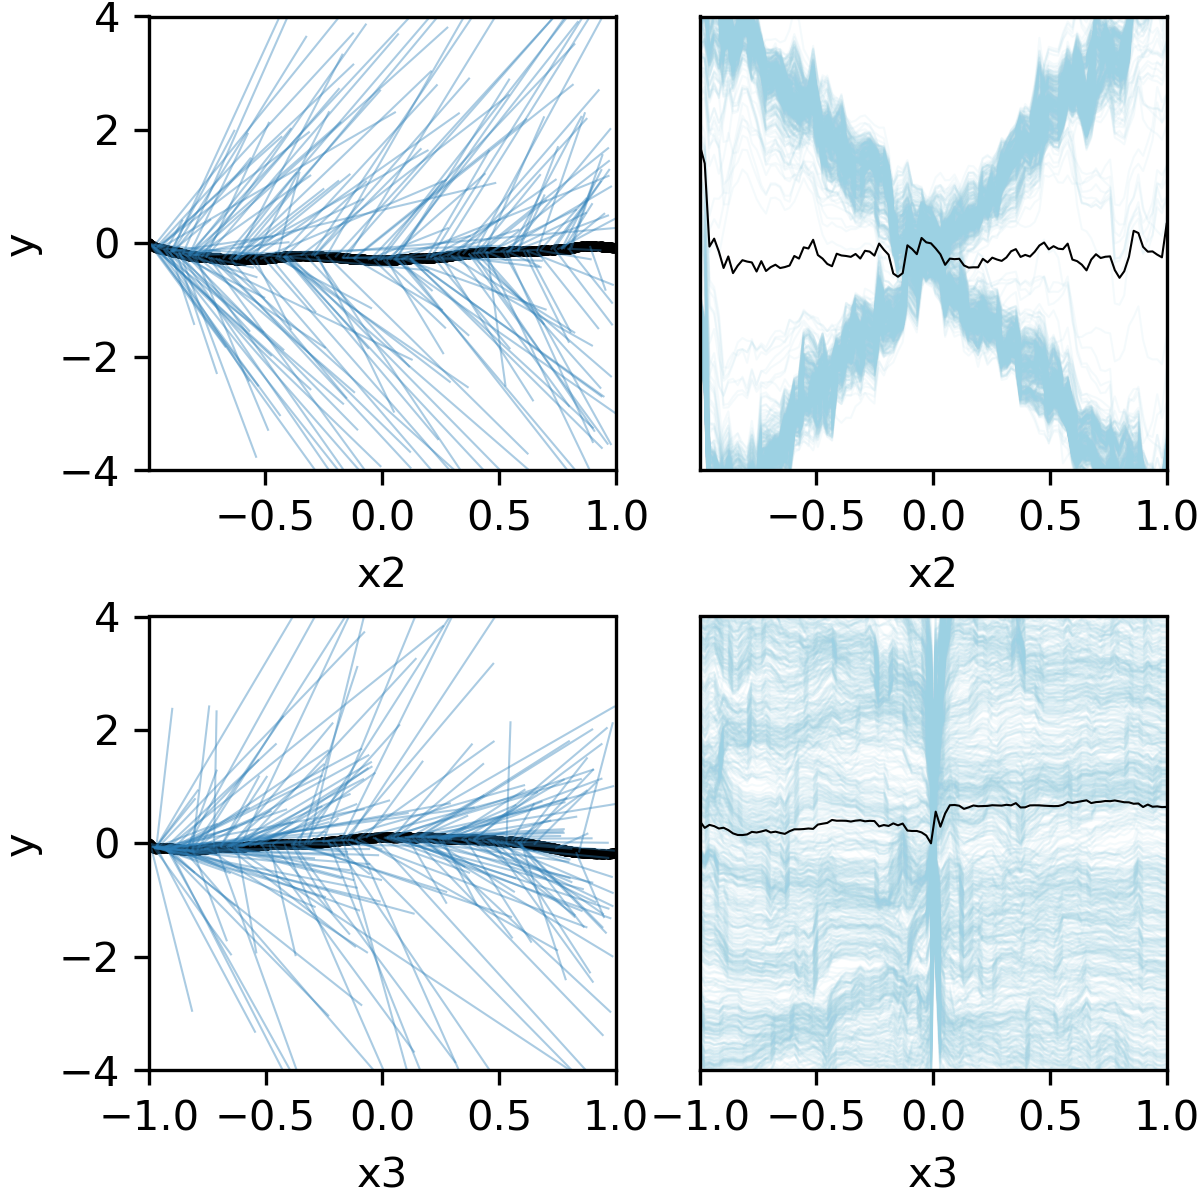
\includegraphics[scale=0.7]{images/bigx.png}
\caption{{\bf big X from ICE}1000 observations}
\label{fig:bigx_stratpd}
\end{subfigure}
\begin{subfigure}[h]{0.495\textwidth}
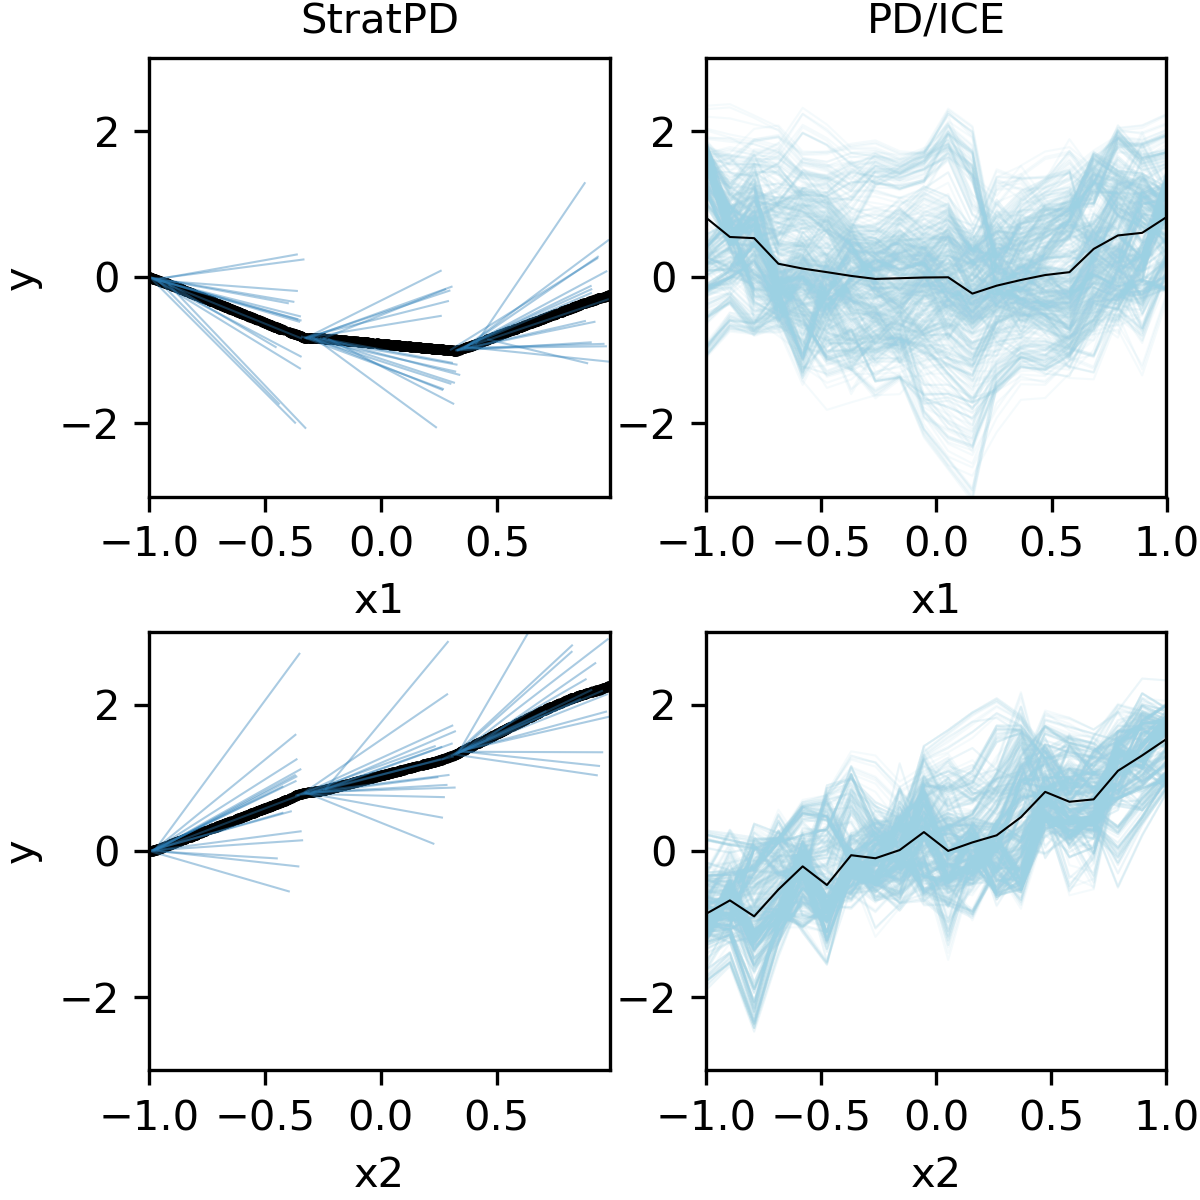
\includegraphics[scale=0.7]{images/additivity.png}
\caption{{\bf additivity from PD/ICE} 1000 observations}
\label{fig:additivity_stratpd}
\end{subfigure}
\end{figure}

The partial dependence curves in the \spd{} and PD/ICE plots for $x_3$ in \figref{fig:bigx_stratpd} are also flat lines because $\frac{\partial y}{\partial x_3}=0$ when $x_3 < 0$ and $10 x_2$ when $x_3 \ge 0$. Since $x_2 \sim U(-1,1)$, $10 x_2$ contributes positive and negative noise to $y$, which the \spd{} plot exhibits with partial derivative lines at random angles.   \todo{James: can you check the ICE paper when they describe that the interactions of $x_3$ are just around 0?  From the equation they are clearly $\ge 0$.}

\cite{ICE} also demonstrate the use of ICE plots for additivity assessment using a second-order equation:

\begin{equation}\label{eq:parabola}
y = x_1^2 + x_2 + \epsilon~~~~~x_1, x_2 \sim U(-1,1), \epsilon \sim N(0,1)
\end{equation}

\noindent We will use this equation to demonstrate that the local, nonparametric method of \spd{} can identify quadratic relationships, as shown in the left column of \figref{fig:additivity_stratpd}; the right column shows the equivalent PD/ICE plots. The \spd{} plots are smoother, but the PD/ICE plot for $x_1$ shows a more accurate parabola with height 1 versus about 0.3 for \spd{}. The amplitude of the $\epsilon$ noise is the same height as the parabola in Equation \eqref{eq:parabola}, which makes it tricky to pick out the quadratic signal.  To smooth out the noise, we set \spd{} hyper parameter ${\it min\_samples\_leaf\_piecewise}$ to 0.5, which means $T'$ partitions $x_c$ space into two $L'$ leaf subregions with roughly half the data. (The default ${\it min\_samples\_leaf\_piecewise}$ is 0.2, meaning look for $L'$ subregions of $x_c$ with 20\% of each $L$'s data.) We examine noise more closely in \secref{sec:noise}.

The effect of $x_2$ on $y$ should be a line with slope 1, as shown in the second row of \figref{fig:additivity_stratpd}. Both PD/ICE and \spd{} plots give accurate depictions of the linear relationship, but \spd{} makes it more clear that the partial dependence of $y$ on $x_2$ is exactly linear.

\subsection{Isolating the effect of codependent features on $y$}\label{sec:codep}

None of the variables used in Equations \eqref{eq:bigX} and \eqref{eq:parabola} are codependent and ICE plots have no problem exposing interactions and generating accurate PD curves.  PD/ICE make the assumption that variables are independent, however, and the plots become less accurate as codependence grows.  To compare \spd{} to PD/ICE for codependent variables, we synthesized a body weight data set with 1000 observations drawn from the following equation with codependence between features.

\begin{equation}\label{eq:weight}
\begin{array}{rll}
y & = &120 + 10(x_{height} - min(x_{height})) + 30x_{pregnant} - 1.5x_{education}\\
\vspace{-10pt}\\
\multicolumn{2}{r}{\text{where}} & x_{sex} \sim Bernoulli(\{M,F\}, p=0.5)\\
                    & & x_{pregnant} = \begin{cases}
                                               Bernoulli(\{0,1\},p=0.5) & \text{ if } x_{sex} = F\\
                                               0 & \text{ if } x_{sex}=M\\
                                               \end{cases}\\
                    & & x_{height} = \begin{cases}
                                               5*12+5+ \epsilon & \text{ if } x_{sex}=F,~ \epsilon \sim U(-4.5,5)\\	
                                               5*12+8 + \epsilon & \text{ if } x_{sex}=M,~ \epsilon \sim U(-7,8)\\
                                               \end{cases}\\
                    & & x_{education} = \begin{cases}
                                               12 + \epsilon & \text{ if } x_{sex}=F,~ \epsilon \sim U(0,8)\\	
                                               10 + \epsilon & \text{ if } x_{sex}=M,~ \epsilon \sim U(0,8)\\
                                               \end{cases}
\end{array}
\end{equation}

\cut{
def toy_weight_data(n):
    df = pd.DataFrame()
    nmen = n//2
    nwomen = n//2
    df['sex'] = ['M']*nmen + ['F']*nwomen
    df.loc[df['sex']=='F','pregnant'] = np.random.randint(0,2,size=(nwomen,))
    df.loc[df['sex']=='M','pregnant'] = 0
    df.loc[df['sex']=='M','height'] = 5*12+8 + np.random.uniform(-7, +8, size=(nmen,))
    df.loc[df['sex']=='F','height'] = 5*12+5 + np.random.uniform(-4.5, +5, size=(nwomen,))
    df.loc[df['sex']=='M','education'] = 10 + np.random.randint(0,8,size=nmen)
    df.loc[df['sex']=='F','education'] = 12 + np.random.randint(0,8,size=nwomen)
}

Because of the codependence between $x_{pregnant}$ and $x_{height}$ via $x_{sex}$, \figref{fig:height_vs_weight} demonstrated that PD/ICE plot incorrectly showed shorter people as heavier on average. PD/ICE conjures up unlikely observation such as pregnant males, resulting in biased ICE lines.

As another example of isolating codependent variable effects, compare the PD/ICE and \spd{} plots in \figref{fig:education_vs_weight} showing number of years of education versus weight. Weight is related to education by slope -1.5, so a perfect partial dependence graph would show a drop of 12 pounds over 8 years of education. The PD/ICE plot captures only about two thirds of that relationship, whereas, the \spd{} plot gets the true education-weight relationship.  Female observations have at least 12 years of education, versus 10 for males, so $x_{education}$ and $x_{sex}$ are codependent, though, there is no interaction term. The fact that women are shorter on average biases the education-weight PD/ICE plot because the baseline weight is lower from which the education contribution is  subtracted.

\begin{figure}[htbp]
\begin{center}
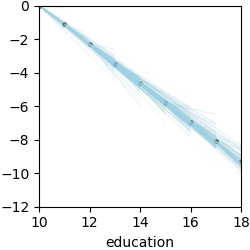
\includegraphics[scale=0.7]{images/education_vs_weight_stratpd.png}
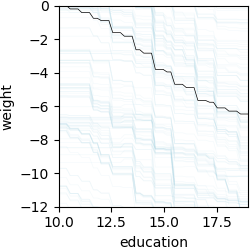
\includegraphics[scale=0.7]{images/education_vs_weight_pdp.png}
\caption{{\bf  educ vs weight}}
\label{fig:education_vs_weight}
\end{center}
\end{figure}

Because the ``signal-to-noise ratio'' is low in the bodyweight data set, we set hyper parameter ${\it min\_samples\_leaf\_partition}=2$. That means to partition \xnc{} into very tight regions, leaving at least two observations from which estimate the change in $y$ over $x_c$ space.

\subsection{The effect of model choice on PD/ICE plots}

Perhaps the biggest issue with PD and ICE plots is that they rely on predictions from a user-provided model $\hat{f}(\bf X)$, and different models make different assumptions and have different strengths and weaknesses.  Users must choose the appropriate model for the data set and properly tune the models, otherwise ICE trendlines are untrustworthy. \figref{fig:4var} shows marginal plots, \spd{} plots, and PD/ICE plots for a 4-variable normal distribution with center $(6, 6, 6, 6)$ and covariance matrix:

\[
\left(
\begin{array}{cccc}
1 & 5 &.7 & 3\\
5 &1 &2 &.5\\
.7 &2 & 1 & 1.5\\
3 &.5 &1.5 &1\\
\end{array}
\right)
\]

\noindent where $y = x_1 + x_2 + x_3 + x_4$.  There are PD/ICE plots from four different models, random forests (100 trees), support vector machines ($\gamma=1/4$), ordinary least squares linear models, and $k$-nearest neighbor ($k=5$).  Because this data set is essentially skewed noise, we increased the number of data points per leaf during $T$ partitioning of \xnc{} and increased $T'$ piecewise partitioning so each leaf contains almost half the $x_c$ data: ${\it min\_samples\_leaf\_partition = 50}$, ${\it min\_samples\_leaf\_piecewise = .4}$.

\begin{figure}[htbp]
\begin{center}
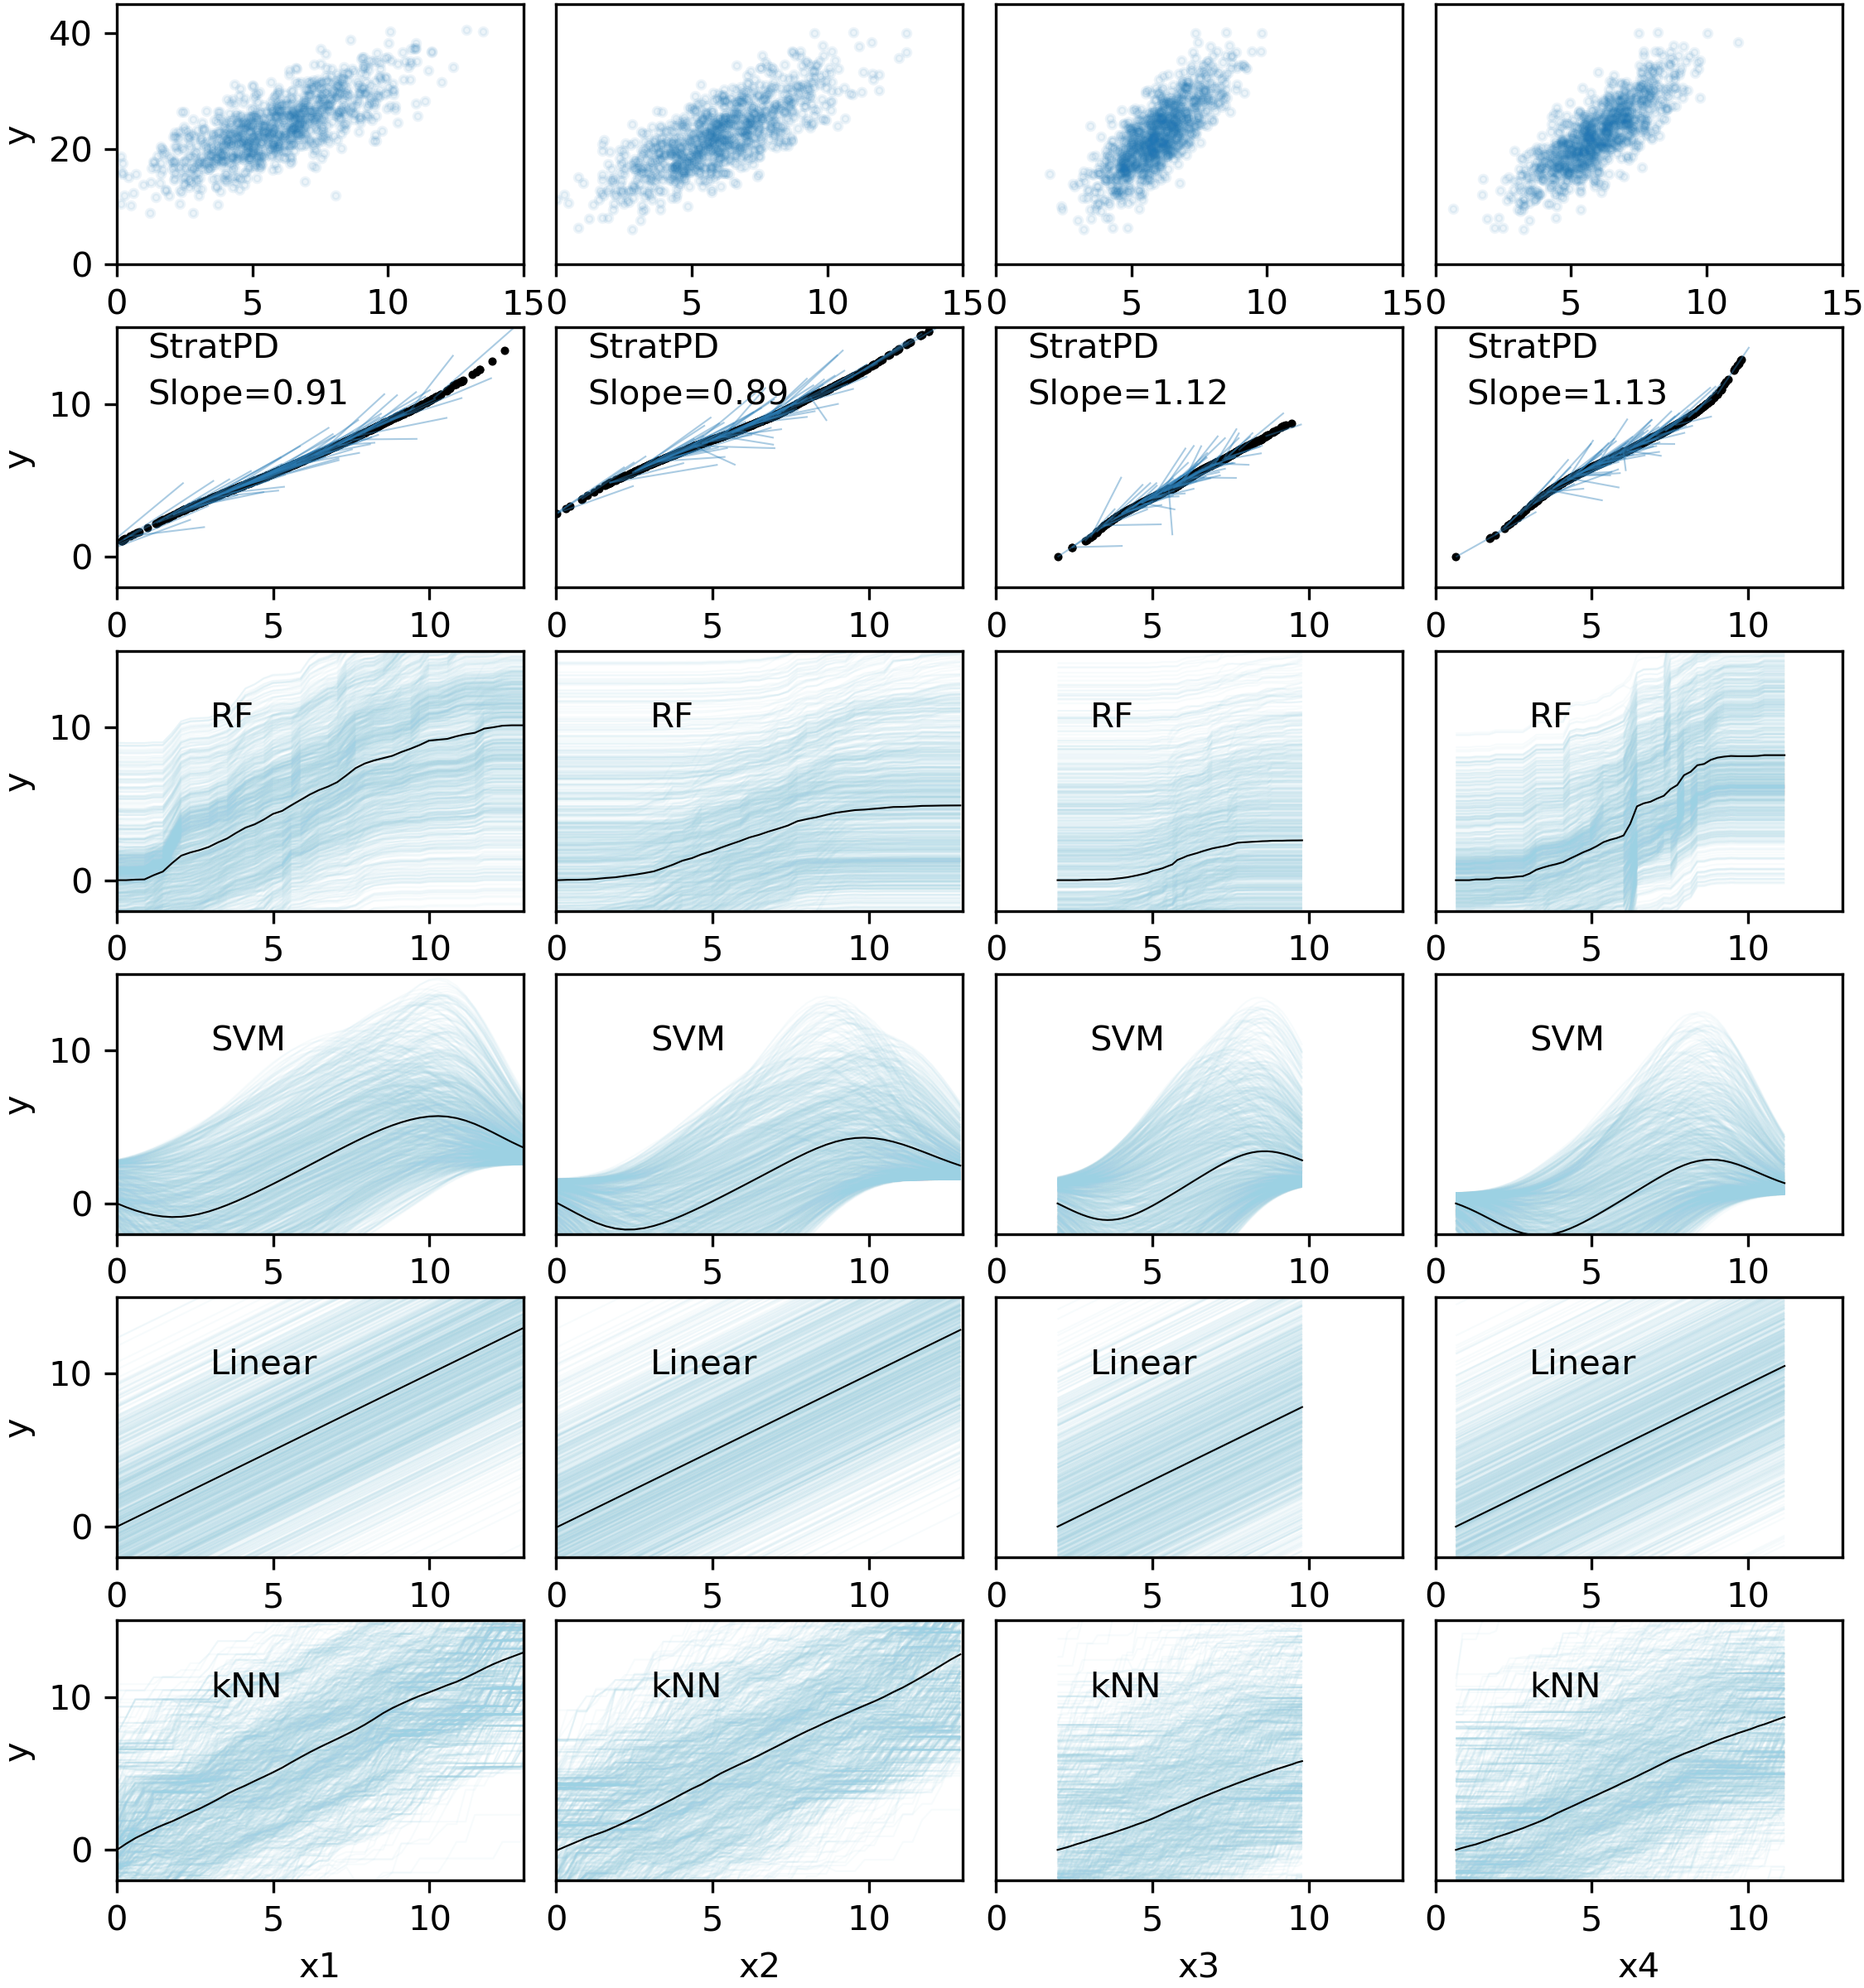
\includegraphics[scale=0.6]{images/multivar_multimodel_normal.png}
\caption{{\bf  multi-model, 4-var gaussian}}
\label{fig:4var}
\end{center}
\end{figure}

Because $\frac{\partial y}{\partial x_{c}} = 1$ for all $x_c$, the partial dependence curves should be lines with slope 1.  The second row of \figref{fig:4var} has \spd{} plots that show linear relationships and the slopes are almost correct.  The PD/ICE plots derived from RF and SVM models show distinct flattening or curving behavior at the edges because the variables are codependent. Models are presented with highly unlikely combinations of $x_i$ variables that are outside of the training data and are forced to extrapolate outside of their support range.  The linear model does very well because it assumes the relationship is linear and, therefore, extrapolates linearly without issue. The nearest neighbor model also captures the linear relationship well but underestimates the partial dependence slope for $x_3$ and $x_4$.
 
\subsection{Duplicated columns require multiple decision trees}\label{sec:dup}

Isolating $x_c$ from codependent variables in \xnc{} through decision tree stratification works well in our experiments unless $x_c$ is a linear function of a variable in \xnc{}. In that case, stratification hammers out variation in $x_c$, as if the decision tree were trained on $(\bf X, y)$ not (\xnc, $\bf y$). To simulate this pathological situation, we duplicated $x_{\it bathrooms}$ from the rent data set and generated the \spd{} and PD/ICE plots in \figref{fig:baths_dup}. \todo{is this where we introduce rent reference citation?} The first column shows plots without a duplicated column and the second column shows the result of duplicating $x_{\it bathrooms}$. Both plots show much reduced partial dependence of $y$ on the highly-predictive variable $x_{\it bathrooms}$. In the case of \spd{}, the stratification process groups the data by apartments with similar bathrooms and so it shows no partial dependence for the duplicated variable.  \todo{why are there many fewer lines in stratpd plot would do begin to column?}

\begin{figure}[htbp]
\begin{center}
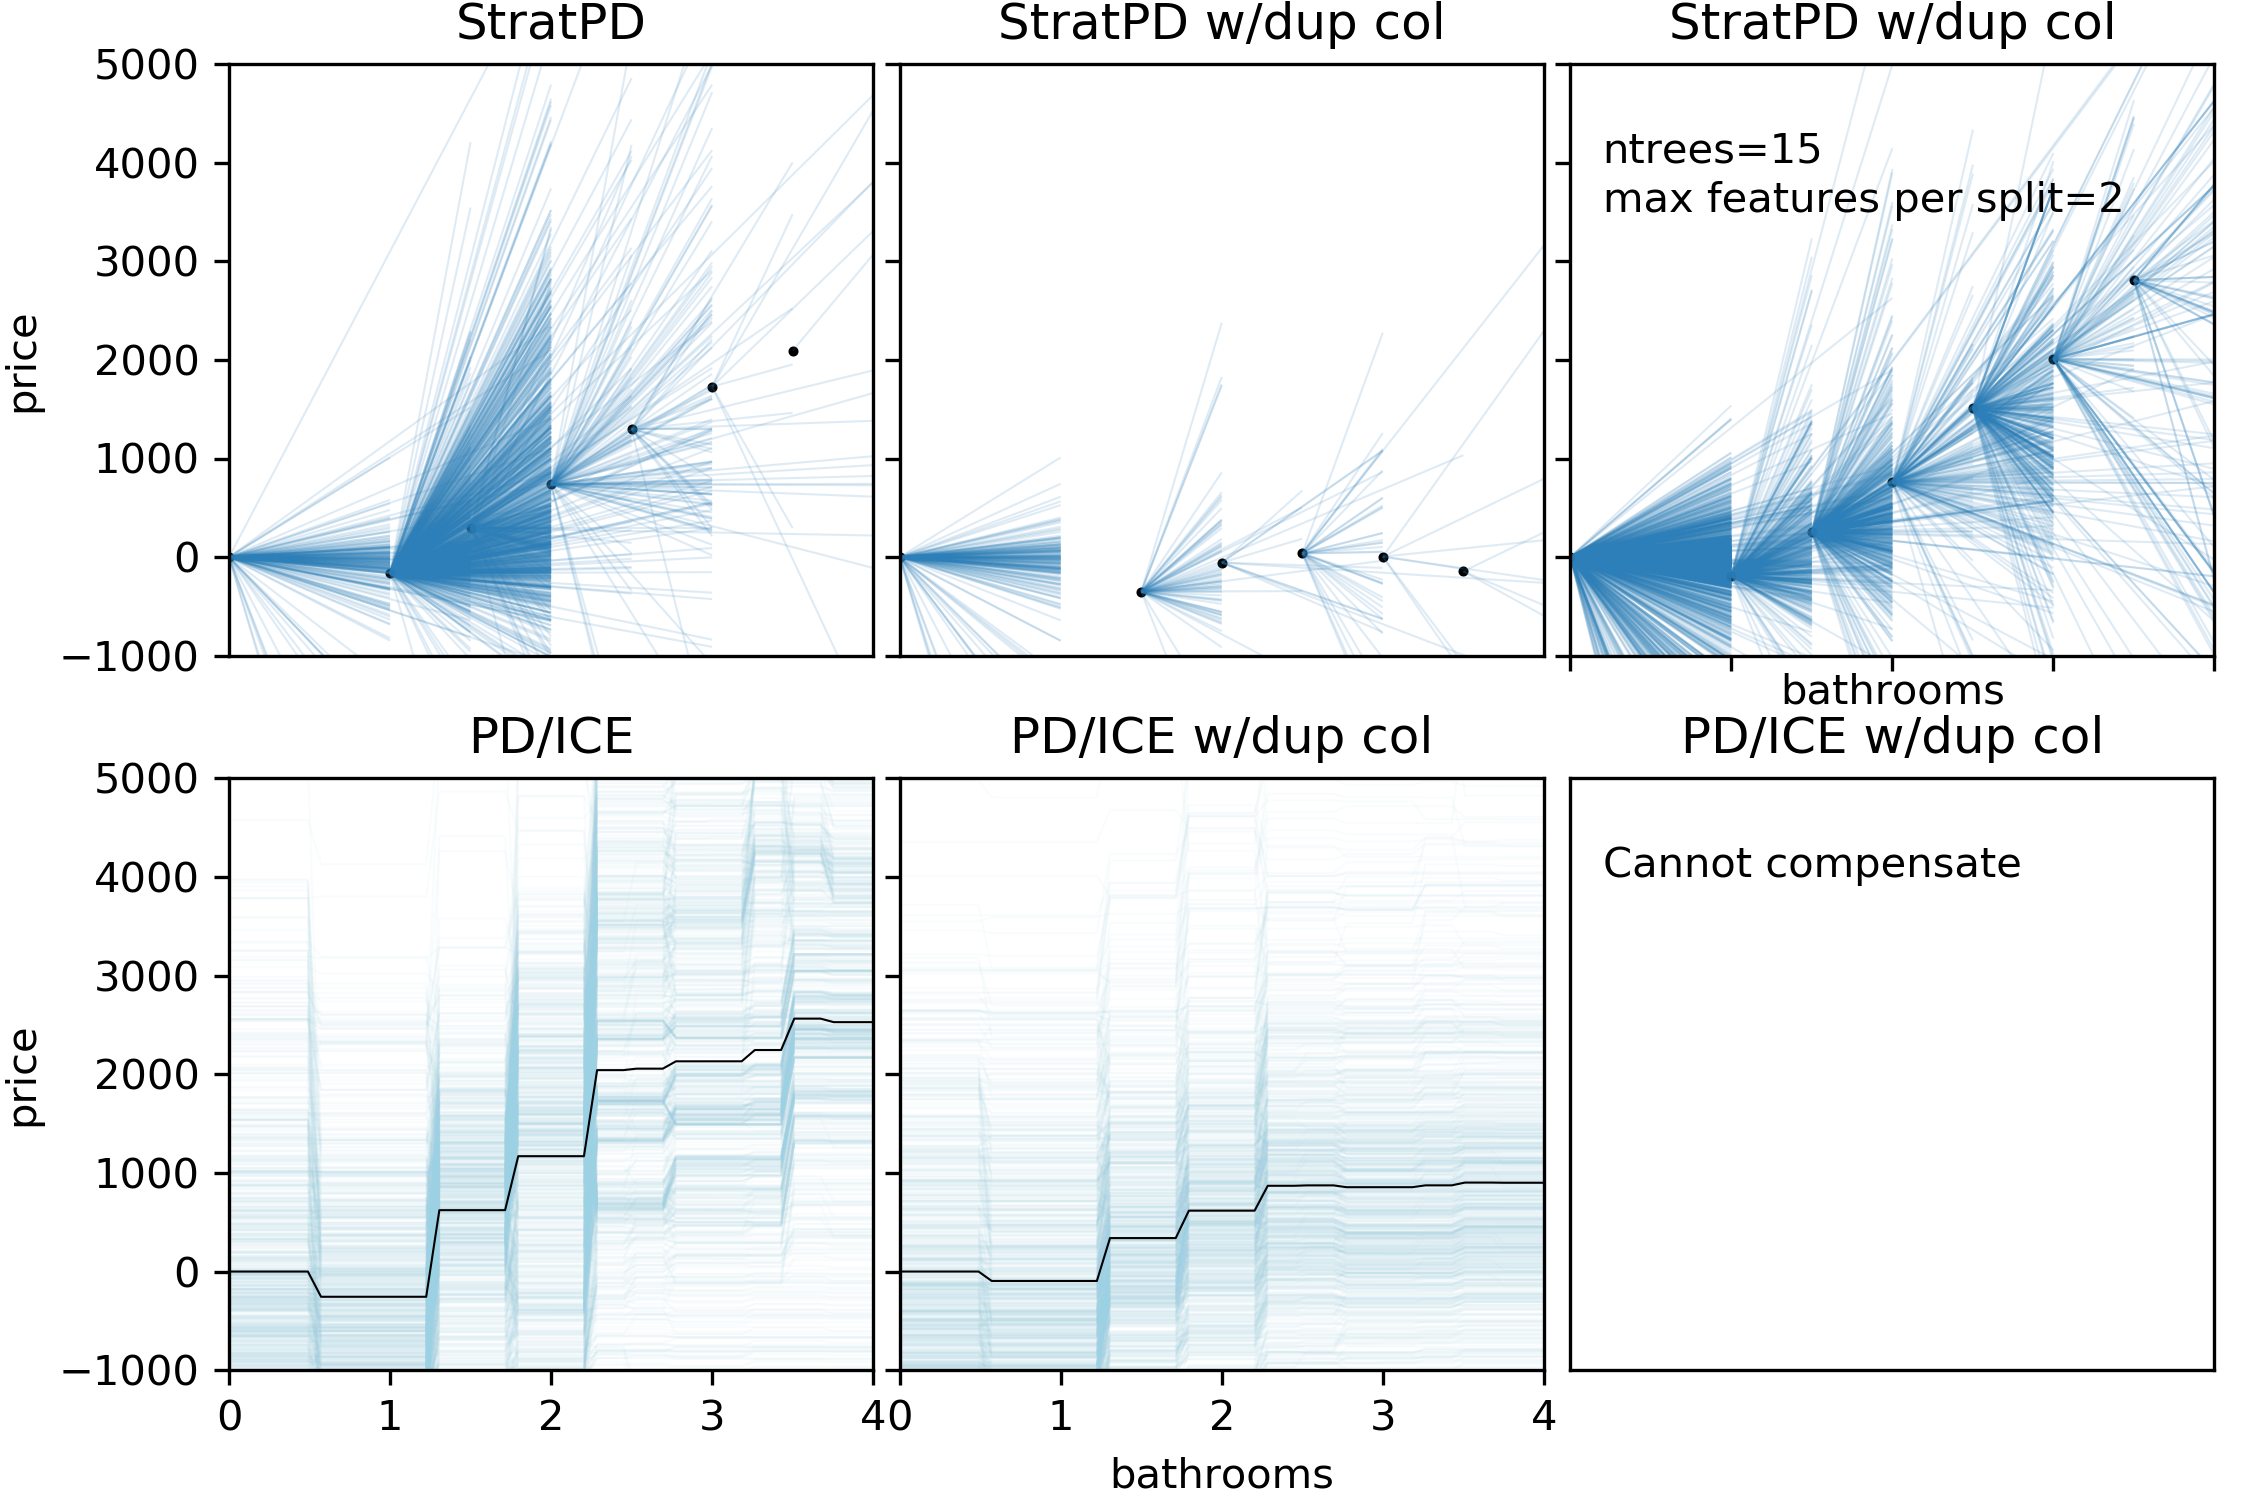
\includegraphics[scale=0.6]{images/bathrooms_vs_price_dup.png}
\caption{{\bf  bathrooms dup col full rent data set (full is 49,353 records. maybe 48k records)}}
\label{fig:baths_dup}
\end{center}
\end{figure}

The problem with the PD/ICE plot is not because of codependence between $x_{\it bathrooms}$ and its duplicate. Instead, that PD/ICE is lower because of the nature of this data set and the way random forests train. With two identical variables, decision nodes that split on one of those variables will choose between them with 50\% probability.  To create ICE trendlines, only one of the duplicate variables changes through $x_{\it bathrooms}$ space, which means that roughly half the tree decision nodes will lead to predictions that ignore the shifted $x_c$ variable.  This has the effect that the model underestimates rent prices.  For example, given an observation with $x_{\it bathrooms}=1$, (simplifying slightly) half the trees in the forest would predict rent appropriate for one bathroom even when the trend line shifts the $x_c$ bathrooms to 4. \todo{James: is this clear enough?}  It would be possible to change the model in an effort to overcome this issue, but many models do not support duplicated or highly-correlated variables.

\cut{
the reason that the ice plot is lowered is due to the data, which has very few data points in the high range of bedrooms. The average is maybe 1.2, so for roughly half the trees, the prediction will be for 1.2 bedrooms no matter what the duplicated bedroom column says.  This problem occurs for strongly predictive features in RF. Linear model couldn't handle duplicate column.}

To compensate for duplicate columns, \spd{} supports the use of random forests rather than a single decision tree to stratify \xnc{} space. The difference from conventional random forest training is that bootstrapping is not important and, in fact, increases bias because the individual trees are working on 2/3 of the data set. The third column, top row in \figref{fig:baths_dup} shows the \spd{} plot resulting from the use of 15 trees ($ntrees=15$) and limiting decision node variable choice to one of two randomly-selected variables at each split (${\it max\_split\_features}=2$).  Restricting the number of variables available during node splitting prevents partitioning from relying too heavily on the duplicate of $x_c$, leading to a number of leaves that vary in $x_c$.

\subsection{Compensating for noise}\label{sec:noise}

To explore the effect of irrelevant variables on \spd{} plots, we introduced a noise column ($x_{\it noise} \sim U(0,50)$) to the rent data set. Because decision trees ignore variables with low predictive power, stratification automatically ignores irrelevant or noise columns.  \figref{fig:beds_noise} shows \spd{} and PD/ICE plots for the original data set and the data set with a noise column. Both approaches are unaffected by the introduction of the noise column, but that is true for PD/ICE because it is derived from a random forest. PD/ICE plots derived from models that are confused by noise columns would not be accurate.

\begin{figure}[htbp]
\begin{center}
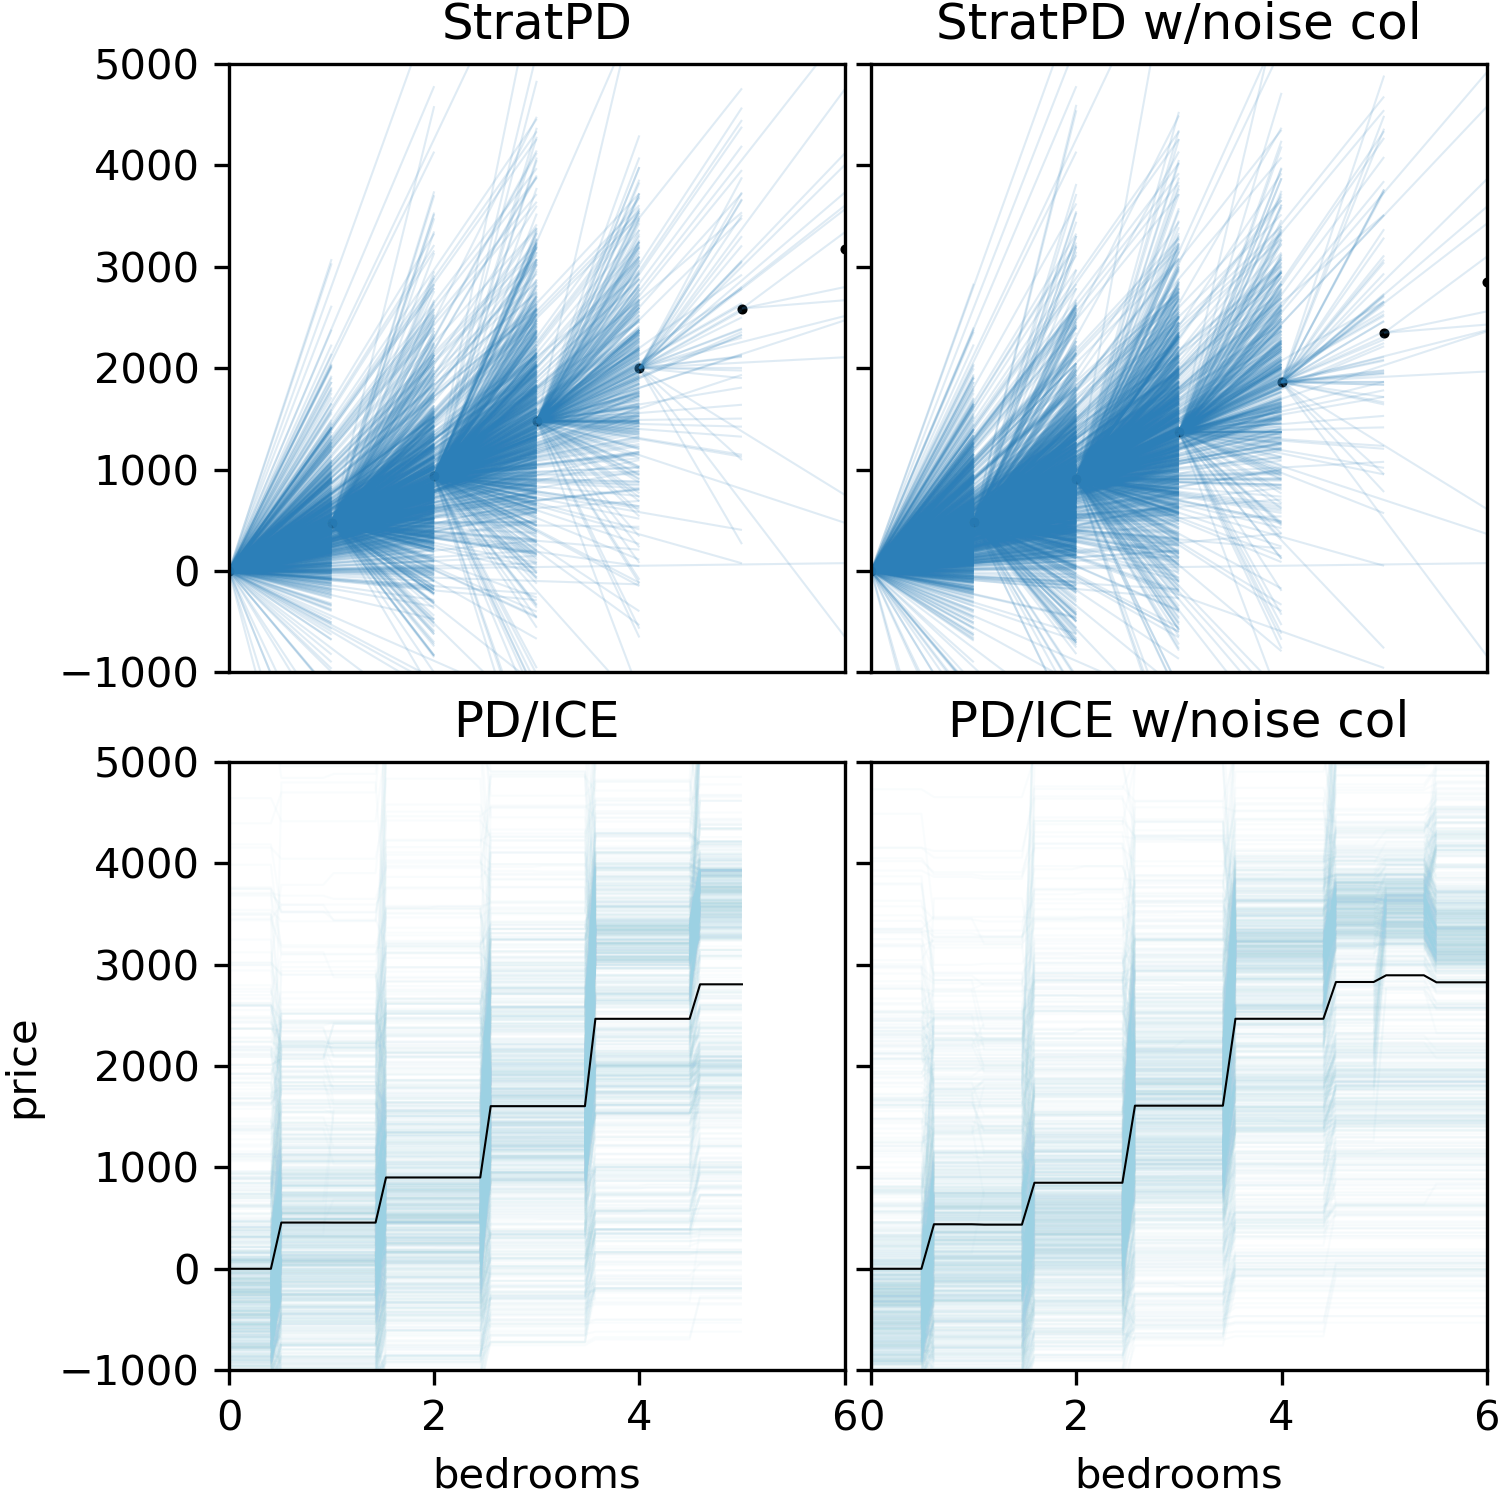
\includegraphics[scale=0.6]{images/bedrooms_vs_price_noise.png}
\caption{{\bf  bedrooms dup col full rent data set (full is 49,353 records. maybe 48k records)}}
\label{fig:beds_noise}
\end{center}
\end{figure}

\begin{figure}[htbp]
\begin{center}
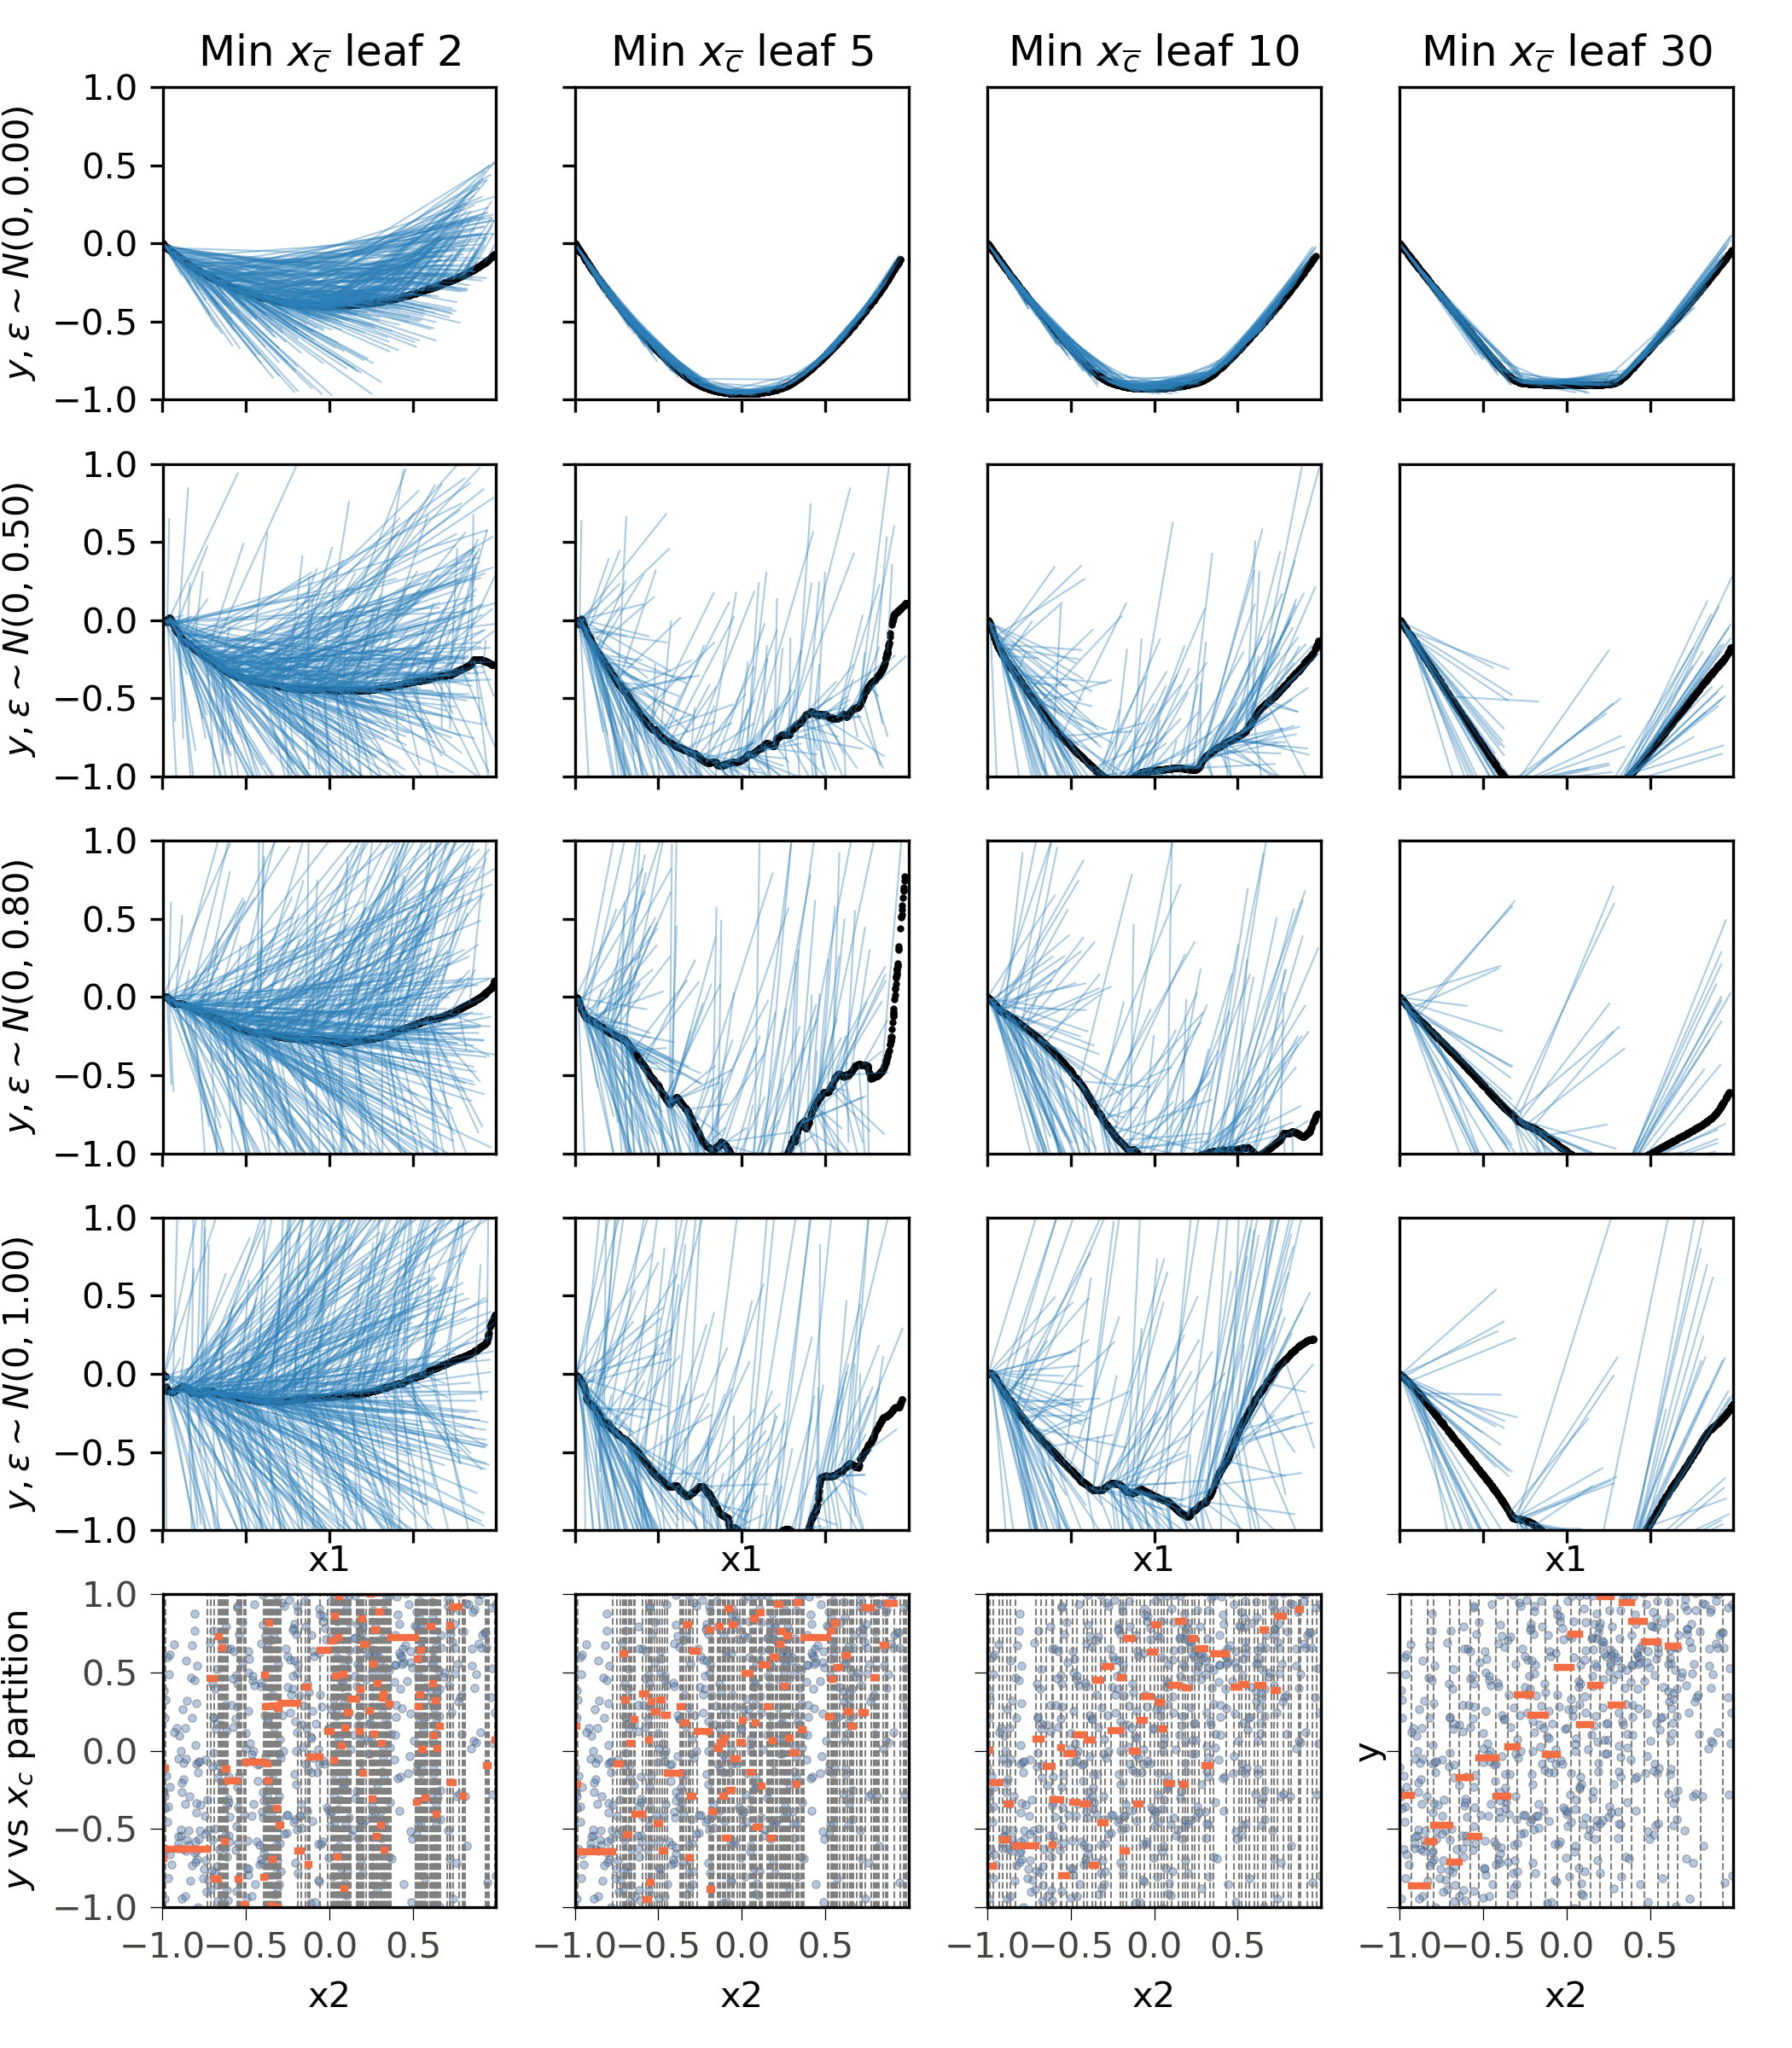
\includegraphics[scale=0.7]{images/meta_additivity_noise.png}
\caption{effect of noise $y = x_1^2 + x_2 + \epsilon$, min leaf size for $x_c=0.3$}
\label{fig:meta_noise}
\end{center}
\end{figure}

Overcoming noisy predictive columns or noisy $y$ sometimes requires hyper parameter tuning. \figref{fig:meta_noise} shows the effect of changing hyper parameter ${\it min\_samples\_leaf\_partition}$ on \spd{} plots at different noise levels for the Equation \eqref{eq:parabola} quadratic data set. The bottom row shows decision tree partitioning of \xnc{}=$x_2$ space. For all plots, hyper parameter ${\it min\_samples\_leaf\_piecewise}$ = .3 (default is .2) to smooth $x_1$. The first row represents the baseline where $y$ omits Gaussian noise.  Increasing the partitioning leaf size for \xnc{}=$x_2$ improves the shape and depth of the parabola, which should be 1.  As more and more Gaussian noise is added to $y$, the \spd{} plots become more erratic, but larger partitioning leaf size tends to compensate.

\subsection{\spd{} and \cspd{} applied to real data} 

We have shown \spd{} operating on a real New York City apartment rent data set, obtained from Kaggle, in figures such as \figref{fig:baths_price} and \figref{fig:rent_ntrees}.  This section shows both \spd{} and \cspd{} plots for another real Kaggle data set, \cite{bulldozer}, concerning auction sales of used bulldozers.  Of the 52 features, we selected three codependent features: YearMade, MachineHoursCurrentMeter, and ModelID. \figref{fig:bulldozer} shows marginal plots for the three variables versus bulldozer sale price in the first column, the \spd{} and \cspd{} plots in the second column, and PD/ICE in the third column. The nominal variable ModelID axis in the third row was sorted by sale price. To reduce overplotting and to reduce ICE plotting time, we use the most recent 10,000 records after dropping those with missing values or zero machine hours. Random forests were trained with 20 not 100 trees but still achieve training set $R^2=0.97$. The  PD/ICE plot for ModelID shows just 1000 of the roughly 1500 unique values (and still takes 6 minutes to generate).

\begin{figure}[htbp]
\begin{center}
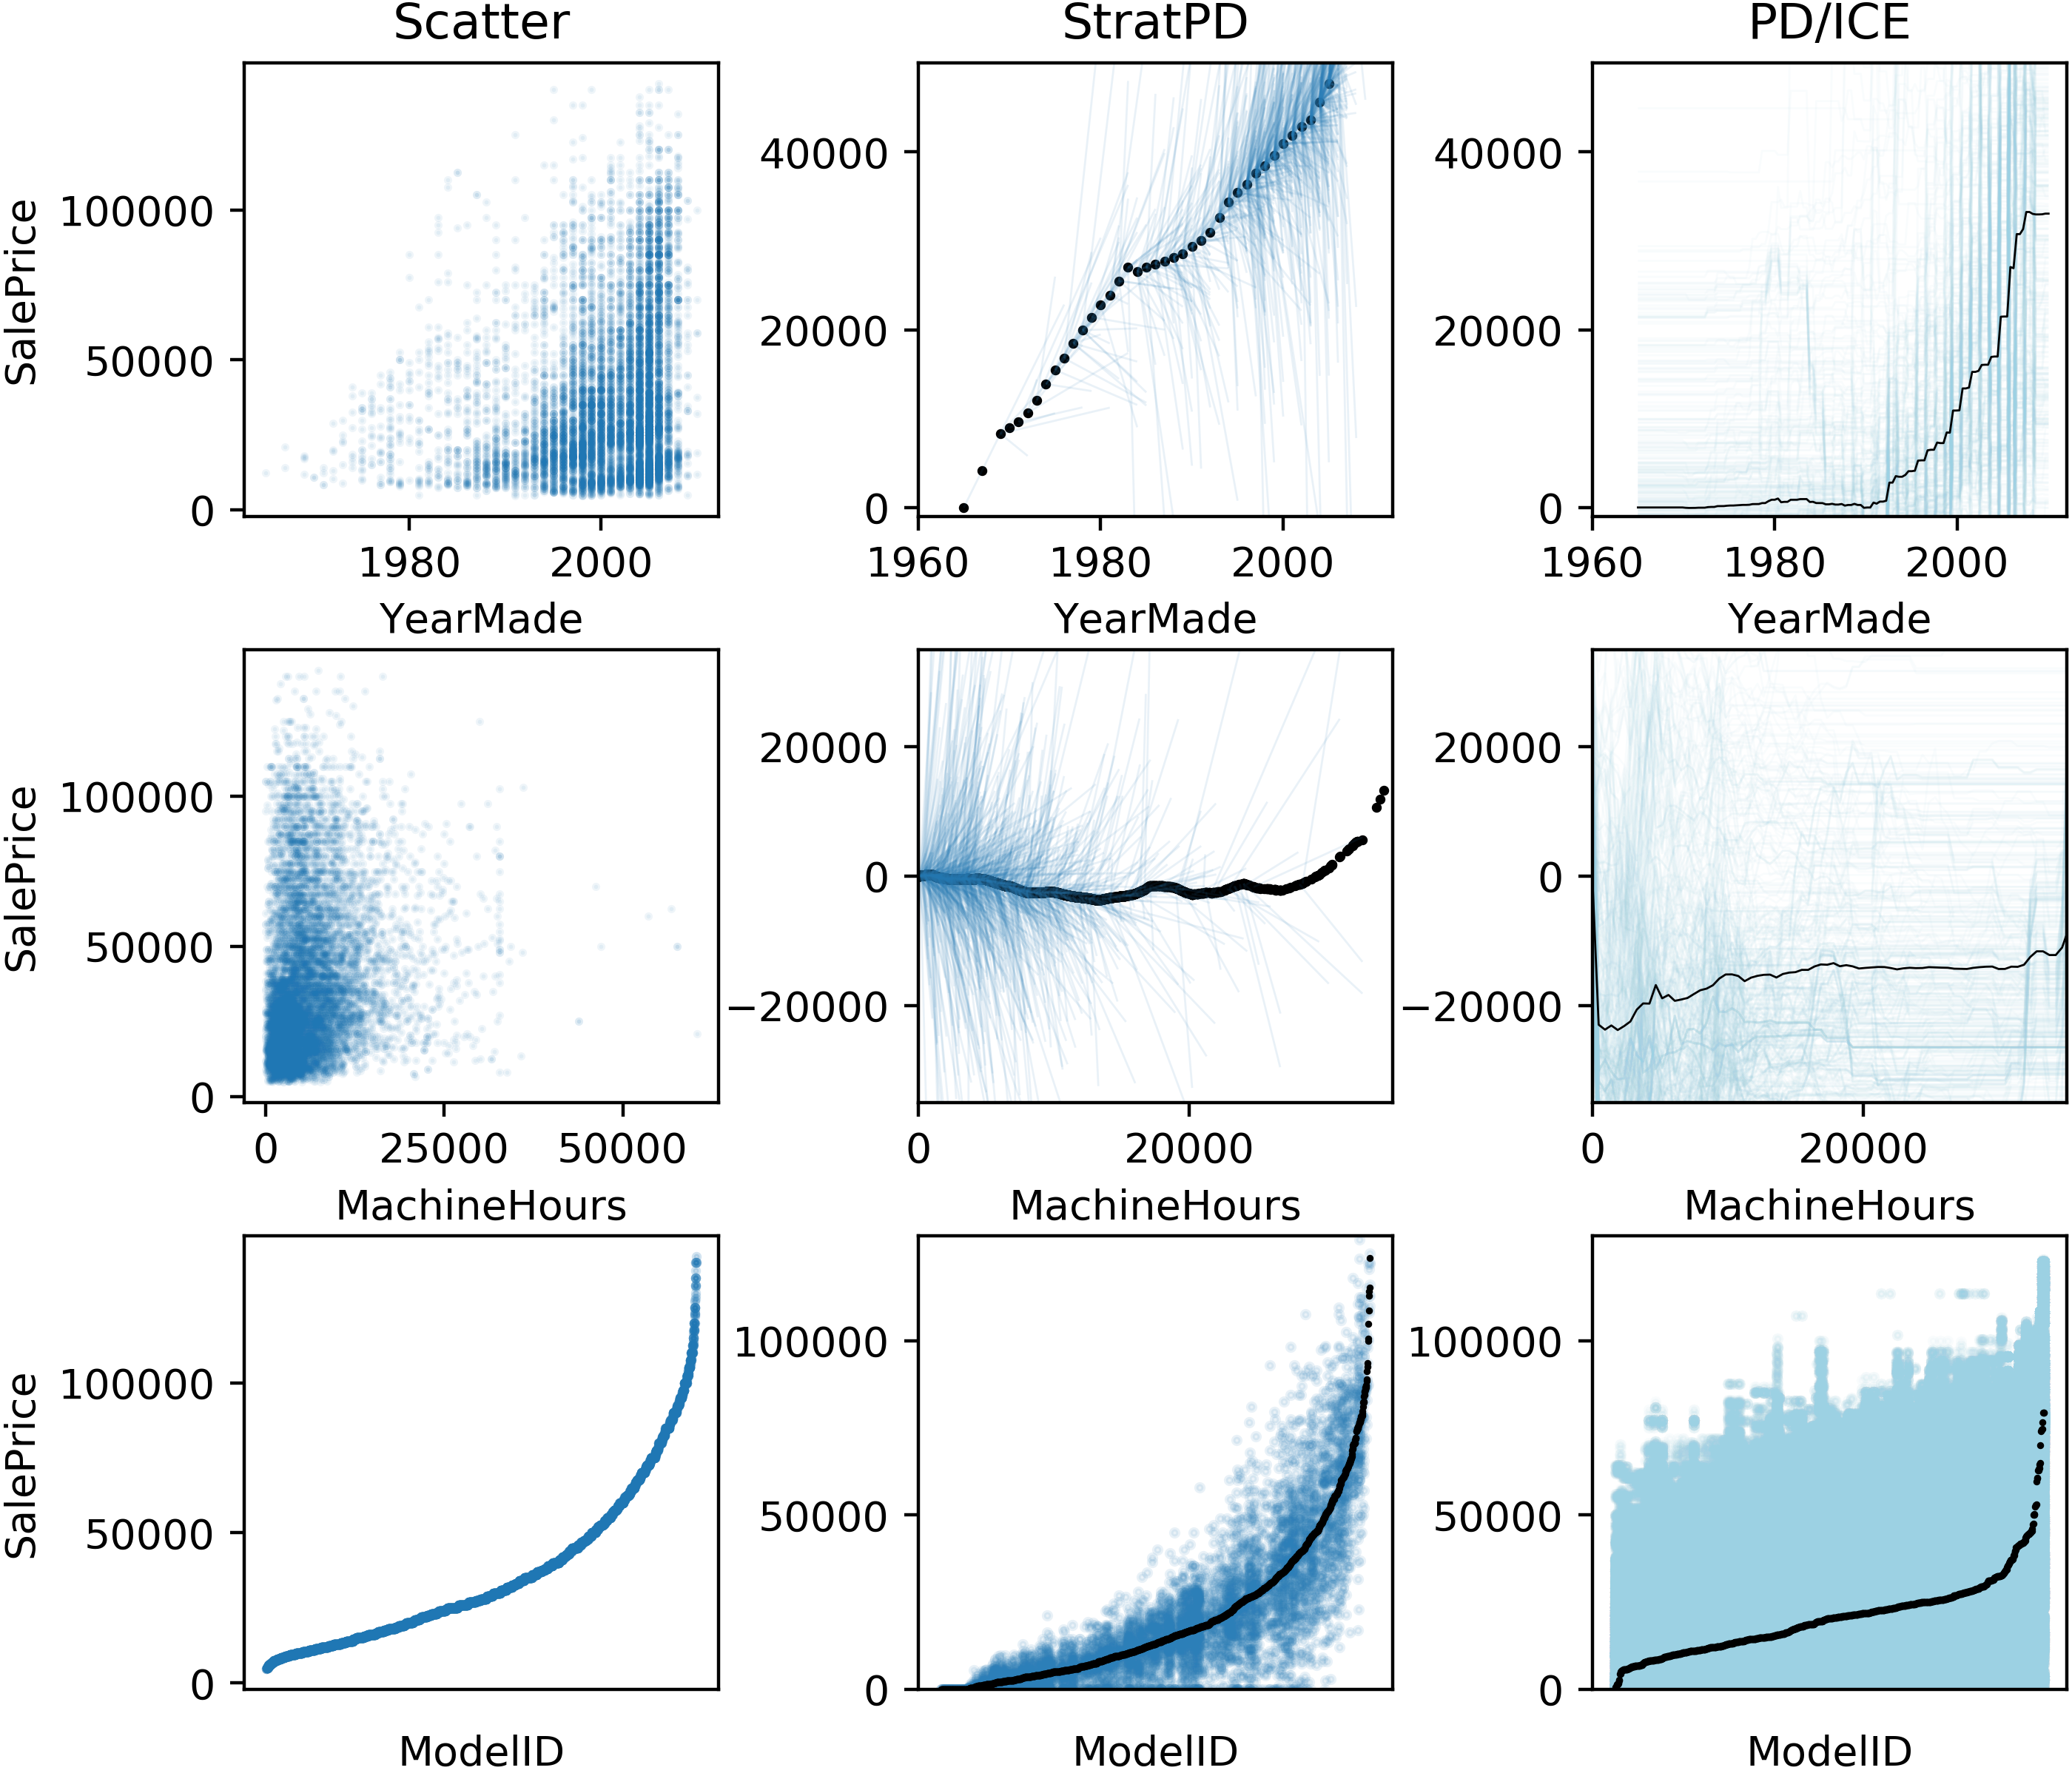
\includegraphics[scale=0.7]{images/bulldozer.png}
\caption{bulldozer; endogeneity, CatStrat Partition RF: missing ModelID training $R^2$ 0.59, Strat Partition RF: missing YearMade training $R^2$ 0.7186, Strat Partition RF: missing MachineHoursCurrentMeter training $R^2$ 0.7714}
\label{fig:bulldozer}
\end{center}
\end{figure}

As this is a real not synthesized data set, the true partial dependence curves are unknown. Further, using only three features means the stratification approach will not be able to cancel out contributions to the sale price from the unused features. (Nontrivial feature engineering would be required to extract predictive features from the other variables and these three get ``out of bag'' $R^2=0.77$) This could be influencing the \spd{} and \cspd{} plots to be more similar to the marginal plots than is correct.

Both the \spd{} and PD/ICE plots show an exponential price decay as bulldozers age, though the \spd{} plot is more of a logit function. It is possible that the slow down in price decay shown in the \spd{} plot is real because it differs significantly from the PD/ICE plot, which will suffer from the codependence of these three features. For example, the ICE lines shift the MachineHours feature into impossible observations, such as bulldozers that have been in use before they were manufactured or bulldozers sold before their ModelID existed. It is clear from both plots that there is a great deal of price variability as bulldozers age.   The \spd{} plot (but not the PD/ICE plot) illustrates that there were many fewer bulldozers for sale that were manufactured before 1990 given the scarcity of lines in that range (which it is consistent with the marginal plot).

The \spd{} plot for MachineHours is flat, indicating no overall change in price as bulldozers get more use.  While counterintuitive, the slope lines indicate a high degree of variability that cancels out, very much like the ``big X'' pattern in \figref{fig:additivity_stratpd}. The PD/ICE plot shows a gradual increase in price as bulldozers get more use, which is highly unlikely, and also shows an immediate drop of about \$30,000 for machines that get used for a few hours. Given that the average bulldozer price is about \$36,000, that initial drop is likely due to variable codependence rather than bulldozers truly losing most of their value immediately.

The \cspd{} plot for ModelID (sorted by sale price) closely matches the marginal plot, which could be the true relationship or due to variables omitted from $\bf X$. The PD/ICE plot also shows that some models are much more expensive than others, but is much more curvilinear. The difference between the plots might mean the \cspd{} plot it is closer to reality because the PD/ICE plots are sensitive to the codependence between the three variables.

\subsection{Pathological partitioning issues}

There are two pathological cases to consider during partitioning, one during \xnc{} and the other during $x_c$ partitioning.  The first case occurs when training yields a decision tree with very large leaves, with perhaps hundreds or thousands of observations.  This can happen when \xnc{} contains a single categorical variable or when the only strongly-predictive variable in \xnc{} is categorical.  The weather data set is a case in point. Choosing $x_c$=$x_{dayofyear}$, means \xnc{}=\{$x_{state}$,$x_{year}$\} and categorical $x_{state}$ accounts for most of the variation in temperature.  \figref{fig:dayofyear_vs_temp}(a) shows the marginal plot of $x_{state}$ versus temperature. A decision tree, $T$, splitting on just $x_{\it state}$, would group all 365 daily temperature observations for a single state into just one leaf. (The marginal plot is showing the complete sine waves but from the side, edge on.)   The \spd{} plot in \figref{fig:dayofyear_vs_temp}(b) clearly shows the sinusoidal temperature fluctuations over the year. The PD/ICE plot also identifies the noisy sine waves, as shown in \figref{fig:dayofyear_vs_temp}(c), but is not smooth as it relies on predictions from a model trained on noisy data. The \spd{} plot is averaging slopes that are themselves smoothing agents.

\begin{figure}[htbp]
\begin{center}
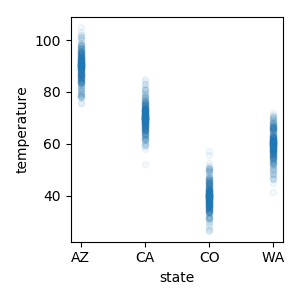
\includegraphics[scale=0.7]{images/state_vs_temp.png}
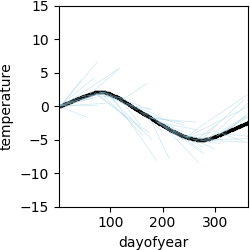
\includegraphics[scale=0.7]{images/dayofyear_vs_temp_stratpd.png}
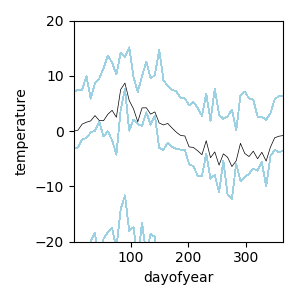
\includegraphics[scale=0.7]{images/dayofyear_vs_temp_pdp.png}
\caption{{\bf  dayofyear  vs temp}}
\label{fig:dayofyear_vs_temp}
\end{center}
\end{figure}

The second partitioning case occurs during piecewise partitioning of $x_c$. Consider the marginal plots in the first column of \figref{fig:rent_intcat} that show the relationship between price and the number of bedrooms and bathrooms. With so many $y$ values for each discrete $x_c$ value, it is highly likely that partitioning $x_c$ will lead to some leaves with unique $x_c$ values. In this situation, it is not possible to detect $y$ changes across $x_c$ and that leaf must be ignored, which means \spd{} throws out data.  Simulations with 10,000-observation subsamples show that \spd{} ignores roughly 5000 observations for $x_c = x_{\it bedrooms}$ and 6500 for $x_c$ = $x_{\it bathrooms}$. 

One way around this problem it is to treat the discrete integers as categories. The third column of \figref{fig:rent_intcat} shows the \cspd{} version derived from the same data. Instead of ignoring roughly 5000 observations, \cspd{} ignores just 25 observations for $x_c = x_{\it bedrooms}$ but still ignores 4900 for $x_c$ = $x_{\it bathrooms}$. The \cspd{} plots are very similar to the \spd{} plots, except in the regions where there is less data.

\begin{figure}[htbp]
\begin{center}
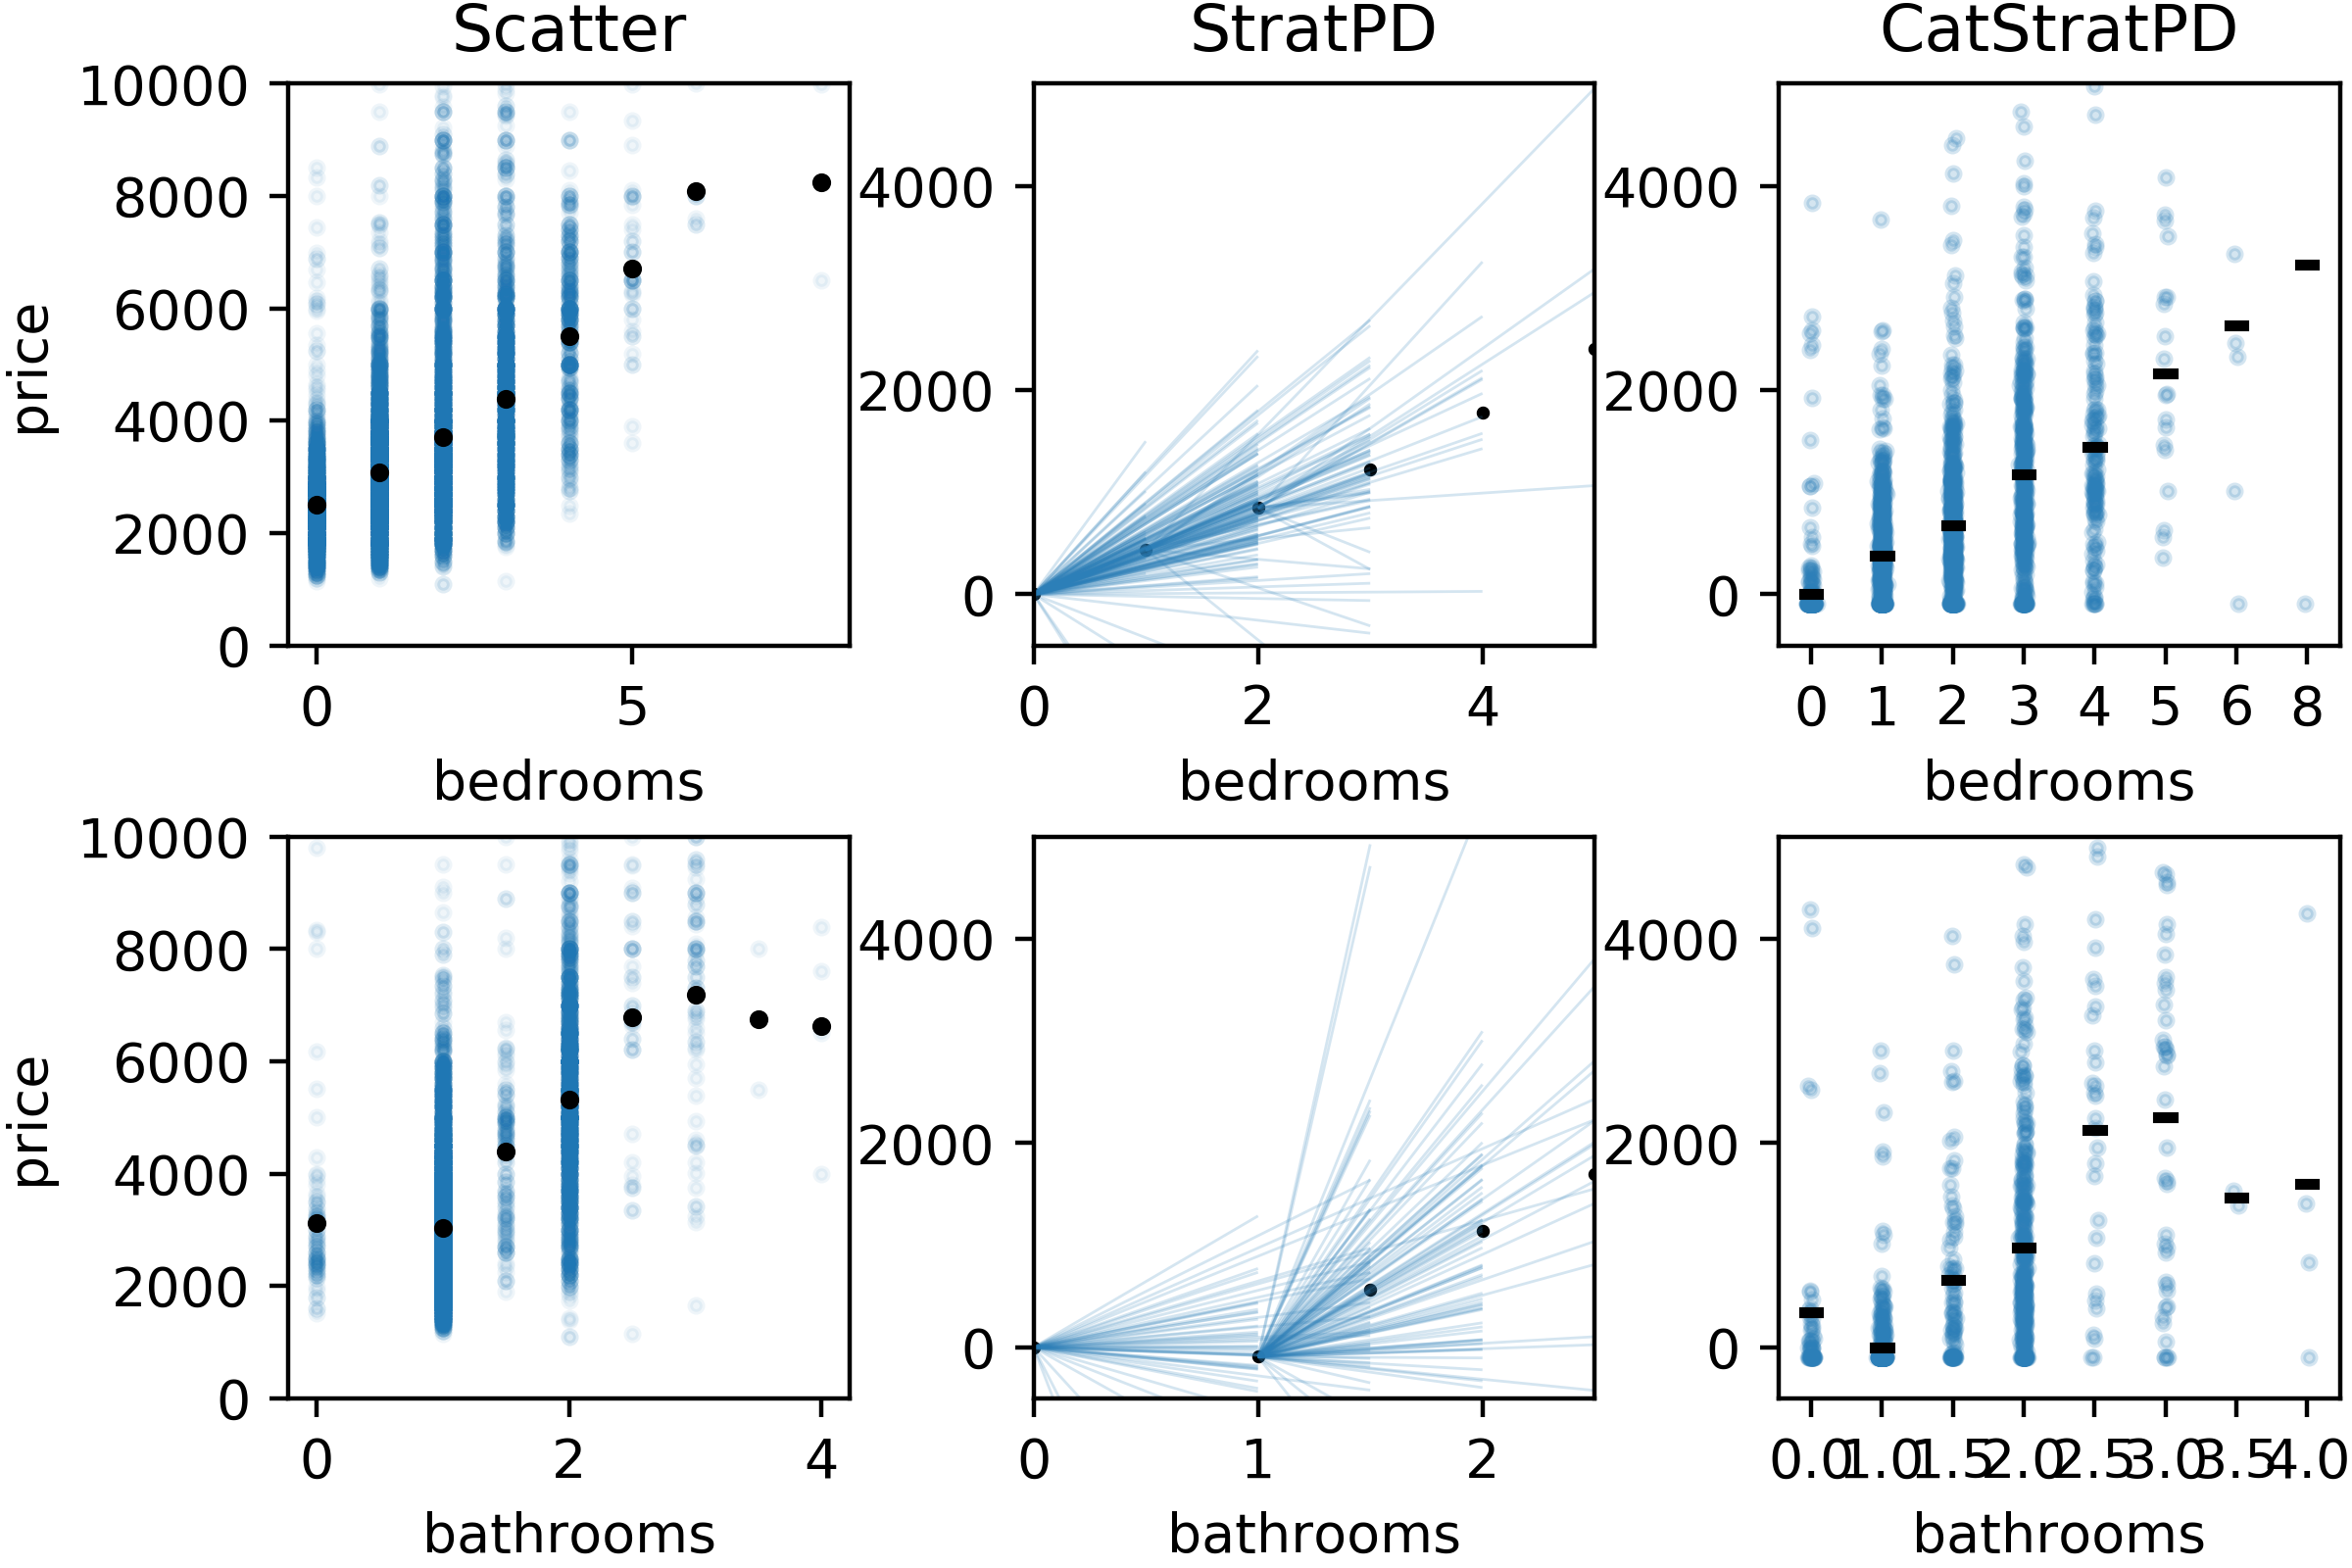
\includegraphics[scale=0.7]{images/rent_intcat.png}
\caption{int cat not usual stratpd}
\label{fig:rent_intcat}
\end{center}
\end{figure}

To further improve the situation, one can increase the default ${\it min\_samples\_leaf\_partition}$ from 10 to 30 to create larger \xnc{} partitions. For $x_c$ = $x_{\it bedrooms}$, \spd{} ignores roughly 4000 and \cspd{} ignores 0 observations and, for $x_c$ = $x_{\it bathrooms}$, \spd{} ignores 3600 and \cspd{} ignores 2155 observations.  Because of the similarity between \spd{} and \cspd{} plots and the stability of the plots under changes to ${\it min\_samples\_leaf\_partition}$, we conclude that the stratification approach works for this data set even when ignoring much of the data.

\subsection{Hyper parameters}

\section{Discussion and Future Work}

can only squash vars in \xnc{} so endogenous vars or vars we don't include that exist end up inflating y. if those vars are codependencies, makes it worse I'd say.

we have just 2 hyper parameters. have Python implementation.

talk about how, since we don't need y to partition, we can partial out the effects of \xnc{} w/o indirection through fallable model.  We examine $x_c$ relationship with $y$ w/o needing model that fits $X$ to $y$, just $x_c$ to $y$. And locally whereas models tend to optimize globally, leading to potentially high bias on average. Emphasize more that we don't go through model, we shoot for $f(\bf X)$.

{\color{red} first re-iterate what we did and the main takeaways}. An important feature of \spd{} is that it directly characterizes the relationship between $\mathbf{y}$ and $x_C$ \emph{without} the need for ever training a machine learning model. In this way \spd{} is {model-independent} and will characterize marginal relationships the same way no matter the user's choice of machine learning algorithm. 

This work describes regressors only, ignoring partial dependence for classifiers.  Research reveals no papers or implementation for classifiers. Friedman, however, briefly describes a partial dependence mechanism for classification whereby $k$-class logistic regression (one-versus-rest) equations indicate the probability of seeing class $k$ at $\bf{x}$.  This suffers from the same interaction-based bias as the regressor model.

better handle on hyper parameters; summarize what we know now.

\section{Conclusion}
\label{sec:conc}

\section{Algorithms}

\setlength{\algomargin}{5pt}
\begin{algorithm}[]
\DontPrintSemicolon
\LinesNumbered
\SetAlgorithmName{Algorithm}{List of Algorithms}
\SetAlgoSkip{}
\SetInd{.5em}{.5em}
\TitleOfAlgo{{\em StratPD}}
\KwIn{$\begin{array}[t]{l}
{\bf X}, {\bf y}, c,\\
{\it ntrees=1}, {\it bootstrap=false}, {\it max\_split\_features=all},\\
{\it min\_samples\_leaf\_partition}, {\it min\_samples\_leaf\_piecewise}\\
\end{array}$
}
\KwOut{collection of $\beta$ coefficients, partial dependence curve}
Train random forest regressor $\it rf$ on (\xnc{}, $\bf y$) with hyper-parameters:\\
~~~~~$\it ntrees$, $\it bootstrap$, $\it max\_split\_features$, ${\it min\_samples\_leaf\_partition}$ \\
\ForEach{tree $T \in \it rf$}{
    \ForEach{leaf $L \in T$}{
    	$(L_x, L_y)$ = $\{(x_{ic},  y_i)\}_{i \in L}$\\
    	Train decision tree regressor $T'$ on $(L_x, L_y)$ with ${\it min\_samples\_leaf\_piecewise}$ \\
    	\ForEach{leaf $L' \in T'$}{
    		$(L'_x, L'_y)$ = $\{(x_{ic},  y_i)\}_{i \in L}$\\
    		$R_{L'}$ = $[min(L'_x), max(L'_x)]$\\
    		\lIf{left$(R_{L'})$ = right$(R_{L'})$}{{\bf continue}}\tcp*[r]{\it Ignore leaves w/o change in $x_c$}
    		Fit linear model to $(L'_x, L'_y)$ giving $\beta_{L'}$\\
    	}
    }
}
$uniqx$ = sorted(unique($x_c$))\\
\For{$i=1$ {\bf to} $|uniqx|-1$}{
	$R$ = $(uniqx_i, uniqx_{i+1})$\\
	\ForEach{leaf $L'$ not ignored from above}{
		$\beta_R = \frac{1}{\Sigma_{L' \in R} |L'|}\Sigma_{L' \in R}|L'|\beta_{L'}$
	}
}
$pd$ = numerically integrate $\beta_R$'s across $uniqx$\\
\Return{collection of all $\beta_R$, $pd$}
\label{alg:StratPD}
\end{algorithm}

\setlength{\algomargin}{5pt}
\begin{algorithm}[]
\DontPrintSemicolon
\LinesNumbered
\SetAlgorithmName{Algorithm}{List of Algorithms}
\SetAlgoSkip{}
\SetInd{.5em}{.5em}
\TitleOfAlgo{{\em CatStratPD}}
\KwIn{$\begin{array}[t]{l}
{\bf X}, {\bf y}, c,\\
{\it ntrees=1}, {\it bootstrap=false}, {\it split\_features=all}, {\it min\_samples\_leaf\_partition}\\
\end{array}$
}
\KwOut{Mapping from category to effect on $y$}
Let $D$ be dictionary mapping category to weighted $\Delta_y$ value\\
Let $S$ be dictionary mapping leaf to leaf size\\
Train random forest regressor $\it rf$ on (\xnc{}, $\bf y$) with hyper-parameters:\\
~~~~~$\it ntrees$, $\it bootstrap$, $\it split\_features$, ${\it min\_samples\_leaf\_partition}$ \\
\ForEach{tree $T \in \it rf$}{
    \ForEach{leaf $L \in T$}{
	$(L_x, L_y)$ = $\{(x_{ic},  y_i)\}_{i \in L}$\\
	$S[L]$ = $\begin{cases} |L| &\mbox{if } |{\it unique~cats \in L_x}| > 1 \\ 
0 & otherwise\end{cases}$\tcp*[r]{\it Assume $L$ is unique id across trees}
	\ForEach{unique $cat \in L_x$}{
		$y_{cat}$ = $L_y[L_x=cat]$\tcp*[r]{\it Group leaf $L_x$ by $cat$, get $y$'s}
		$\overline{y}_{cat}$ = $mean(y_{cat})$\tcp*[]{\it $\overline{\bf y}$ is list of cat means}
	}
	\ForEach{unique $cat \in L_x$}{
		$\Delta y_{cat} = \overline{y}_{cat} - {min}(\overline{\bf y})$\tcp*[r]{\it Strip \xnc{}'s y contribution}
		$D[cat] = D[cat] + \Delta y_{cat} \times S[L]$\tcp*[r]{\it Accumulate weighted $\Delta_y$'s for each $cat$}
	}
   }
}
$n = \Sigma_{T \in {\it rf}} \Sigma_{L \in T}S[L]$\tcp*[r]{\it Num observations used to compute averages}
$D[cat] = \frac{1}{n} D[cat]$\tcp*[r]{\it Get average of leaf averages for $cat$}
$D[cat] = D[cat] - min(D)$\tcp*[r]{\it Normalize lowest $D[cat]$ to 0}
\Return{$D$}
\label{alg:CatStratPD}
\end{algorithm}

\newpage
\bibliographystyle{apalike}

\bibliography{stratpd}
\end{document}